\documentclass[11pt, final]{beamer}

\usepackage[utf8]{inputenc}
\usepackage[T1]{fontenc}

% Graphics
\usepackage{graphicx}
\usepackage{tikz}
\usepackage{pgfplots}

% Language localization
\usepackage[english]{babel}

% Symbols
\usepackage{amsmath}
\usepackage{amsfonts}
\usepackage{amssymb}

% Bold math style, useful for vectors
\usepackage{bm}

% For supressing caption "Figure X" text
\usepackage{caption}

\usepackage{ulem}

\usepackage{subcaption}

\usepackage{todonotes}

\usetheme{Madrid}
\setbeamertemplate{navigation symbols}{}

\begin{document}
	
	% Add typographic commands
	\newcommand{\mrm}[1]{\mathrm{#1}}
	\newcommand{\eu}{\mrm{e}}
	\newcommand{\iu}{\mrm{i}}	
	
	%%%%%%%%%%%%%%%%%%%%%%%%%%%%%%%%%%
	% Räkna 5 min bakgrund, 6 min teori, 6 min simuleringar, 3 min diskussion
	%%%%%%%%%%%%%%%%%%%%%%%%%%%%%%%%%%
	\author{Niklas Wingren}
	\title[Acousto-Electromagnetic Interaction]{Acousto-Electromagnetic Interaction in Materials for Aerospace Composites}
	\subtitle{Master's Thesis in Electrical and Information Technology}
	\date{2019-01-29}
	\frame[plain]{\maketitle}
	
	\begin{frame}{Overview}
		\tableofcontents
	\end{frame}
	
	\AtBeginSection[]{
		\begin{frame}{Overview}
			\tableofcontents[currentsection]
		\end{frame}
	}
	
	\section{Background}
	
	\begin{frame}{Background}{Composites in aerospace}
		\begin{itemize}
			\item Composite materials attractive in aerospace due to light weight, high strength, no corrosion and more
			\begin{figure}
				\includegraphics[width=0.4\textwidth]{Glare_honeycomb.jpg}
			\end{figure}
			\pause
			\item Non-destructive testing (NDT) is a crucial part of manufacturing and servicing
			\item Detection and evaluation of flaws in material without negative effects
			\pause
			\item Many methods
			\begin{itemize}
				\item Ultrasonic testing
				\item Microwave/mm-wave imaging
			\end{itemize}
		\end{itemize}
		
	\end{frame}
	
	\begin{frame}{Background}{Combination of methods}
		\begin{itemize}
			\item Combination of methods might give improved detection
			\item Knowledge on possible interaction mechanisms required
			\pause
			\item Purpose of thesis
			\begin{itemize}
				\item Investigate mechanisms behind acousto-electromagnetic interaction
				\item Identify relevant properties of the wave phenomena
				\item Could this be used to improve NDT?
			\end{itemize}
		\end{itemize}
	\end{frame}
	
	\begin{frame}{Background}{Acousto-optics}
		\begin{columns}
			\begin{column}{0.6\textwidth}
				\begin{itemize}
					\item<1-> Interaction between ultrasound and laser
					\item<1-> Ultrasonic wave causes periodic perturbation in refractive index
					\item<2-> Phase matching at specific condition (Bragg condition)
					\begin{equation*}
						\sin{\theta_B} = \frac{\lambda}{2\Lambda}
					\end{equation*}
					\item<3-> Used in photonics for manipulation of laser beams
				\end{itemize}
			\end{column}
			\begin{column}{0.4\textwidth}
				\uncover<2->{
					\resizebox{\textwidth}{!}{
						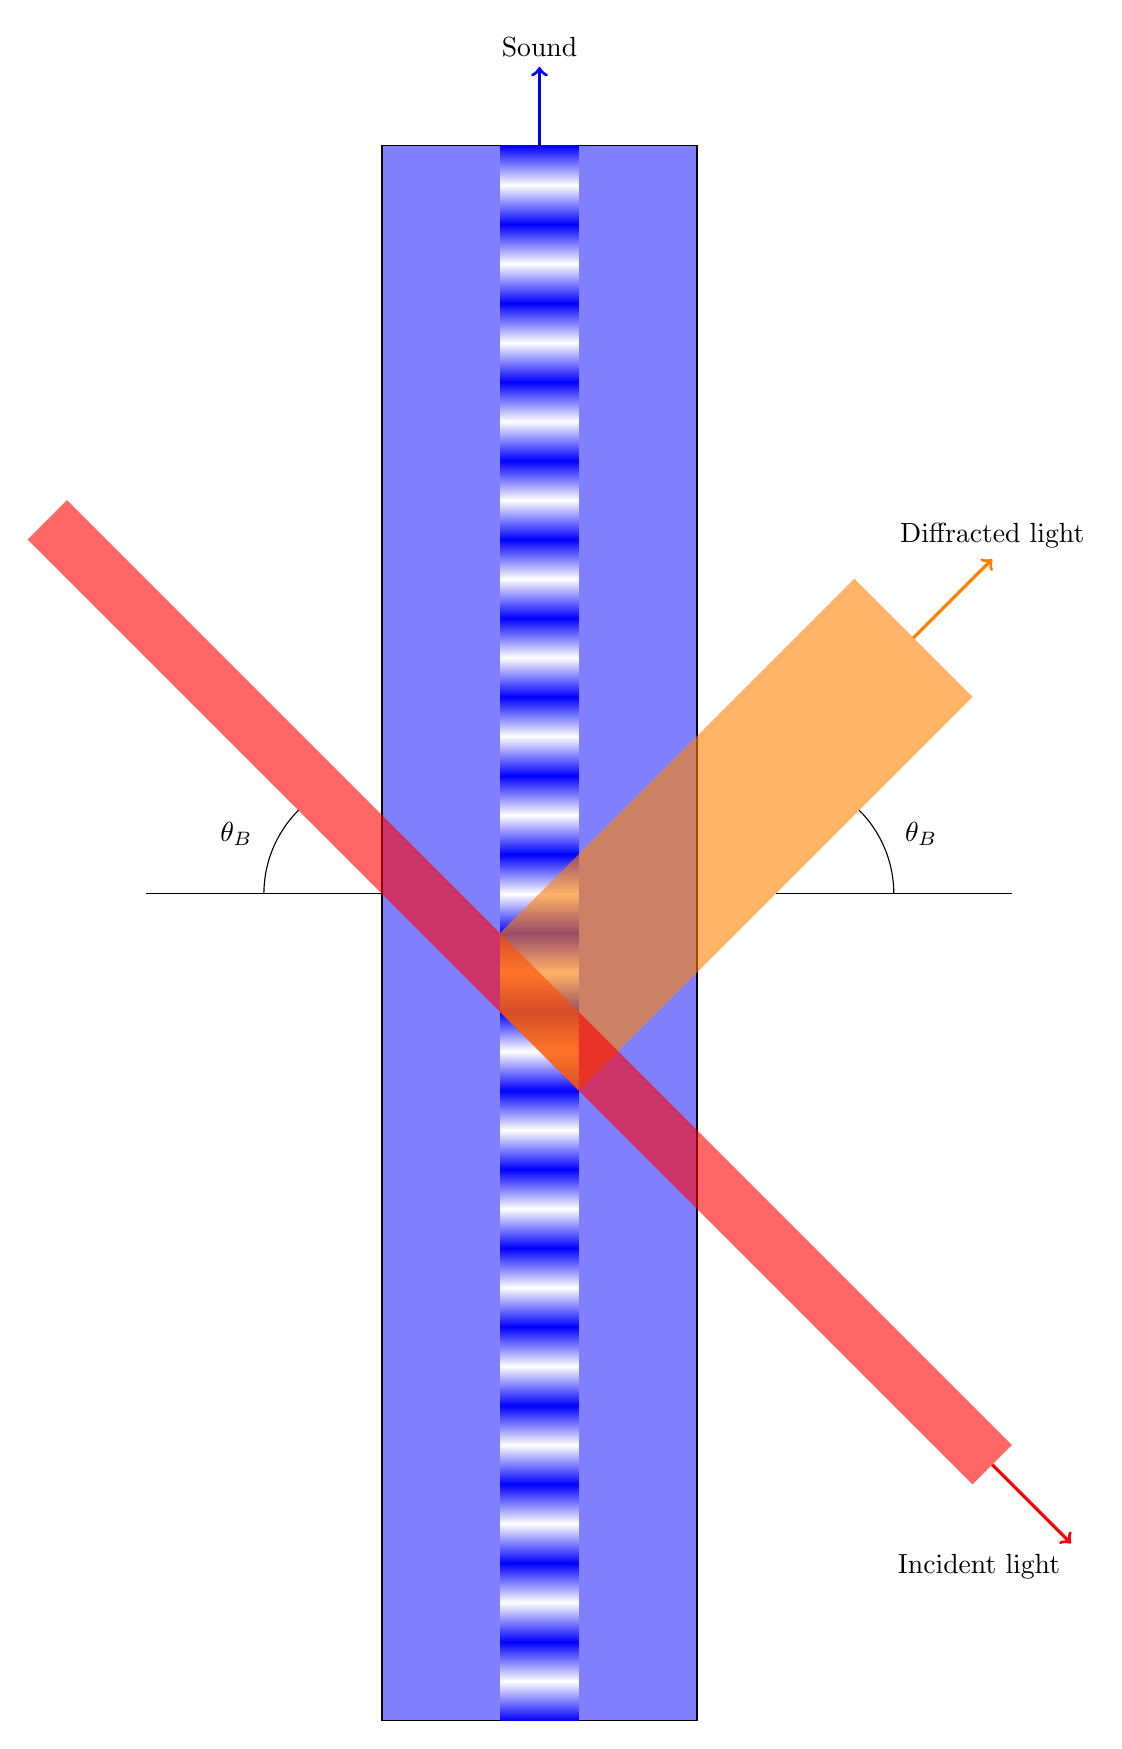
\begin{tikzpicture}
	\draw[fill=blue!50!white] (-2,0) rectangle ++(4,20);
	\foreach \i in {0,1,...,39}
		\path [bottom color=blue, top color=white, shading angle = {mod(\i,2)*180}]
		(-0.5,{\i/2}) rectangle ++(1,0.5);
		
	\fill[red,opacity=0.6] (-6.5,15) -- ++(7,-7) -- (0.5,9) -- ++({-7+sqrt(0.5-0.5*0.5)},7-0.5);
	\fill[orange,opacity=0.6] (0.5,8) -- ++(5,5) -- ++({-sqrt(4.5-1.5*1.5)},1.5) -- (-0.5,10) -- (-0.5,9);
	\fill[red,opacity=0.6] (0.5,8) -- ++(5,-5) -- ++({sqrt(0.5-0.5*0.5)},0.5) -- (0.5,9);
	
	\draw[->,blue,very thick] (0,20) -- (0,21) node[anchor=south,text=black]{Sound};
	\draw[->,orange,very thick] ({5.5-sqrt(4.5-1.5*1.5)+sqrt(1.5*1.5/2-0.75*0.75)},13.75) -- ++(1,1) node[anchor=south,text=black]{Diffracted light};
	\draw[->,red,very thick] ({5.5+sqrt(0.5-0.5*0.5)-sqrt(0.5*0.5/2-0.25*0.25)},3.25) -- ++(1,-1) node[anchor=north east,text=black]{Incident light};
	
	\draw (-2,10.5) -- ++(-3,0);
	\draw[shift={(-2,10.5)}] ([shift={(180:1.5)}] 0,0) arc(180:135:1.5) (157.5:2) node{$\theta_B$};
	\draw (3,10.5) -- ++(3,0);
	\draw[shift={(3,10.5)}] ([shift={(0:1.5)}] 0,0) arc(0:45:1.5) (22.5:2) node{$\theta_B$};
\end{tikzpicture}
					}
				}
			\end{column}
		\end{columns}
	\end{frame}
	
	\begin{frame}{Background}{RASS}
		\begin{itemize}
			\item Radio Acoustic Sounding System
			\item Meteorological method for measuring atmospheric teperature
			\pause
			\item Interaction mechanism is the same as in acousto-optics
			\item Frequency order of magnitude: audible sound and radio (MHz - GHz)
		\end{itemize}
	\end{frame}
	
	\section{Theory}
	
	\begin{frame}{Theory}{Photoelasticity}
		\begin{itemize}
			\item Strain in material affecting dielectric properties
			\pause
			\item Simple photoelastic model
			\begin{equation*}
				\varepsilon = \varepsilon_0 (\varepsilon_\mrm{r} + \varepsilon_1), \qquad \varepsilon_1 = \frac{\varepsilon_\mrm{r}^2 \mathfrak{p}}{K} \,p
			\end{equation*}
			\begin{equation*}
				\mathfrak{p} = \frac{(\varepsilon_\mrm{r} - 1)(\varepsilon_\mrm{r} + 2)}{3\varepsilon_\mrm{r}^2}
			\end{equation*}
			\pause
			\item Dielectric perturbation proportional to acoustic pressure
		\end{itemize}
	\end{frame}
	
	\begin{frame}{Theory}{Scattering against dielectric perturbation}
		\begin{itemize}
			\item Maxwell's equations
			\begin{align*}
				&\nabla \times \bm{E} = \iu\omega \mu_0 \bm{H} - \mu_0 \frac{\partial \bm{H}}{\partial t} \\
				&\nabla \times \bm{H} = -\iu\omega \varepsilon \bm{E} + \mu_0 \frac{\partial (\varepsilon \bm{E})}{\partial t} \\
				&\nabla \cdot (\varepsilon \bm{E}) = 0 \\
				&\nabla \cdot \bm{H} = 0
			\end{align*}
			\pause
			\item Small dielectric perturbation $\varepsilon_1$
			\begin{equation*}
				\varepsilon = \varepsilon_0(\varepsilon_\mrm{r} + \varepsilon_1)
			\end{equation*}
			\item Electric field divided into incident and small scattered field
			\begin{equation*}
				\bm{E} = \bm{E}_\mrm{i} + \bm{E}_\mrm{sc}
			\end{equation*}
		\end{itemize}
	\end{frame}
	
	\begin{frame}{Theory}{Scattering against dielectric perturbation}
		\begin{itemize}
			\item Inhomogeneous Helmholtz equation
			\footnotesize
			\begin{equation*}
				\nabla^2\bm{E}_\mrm{sc} + k^2 \bm{E}_\mrm{sc} =	-k^2 \frac{\varepsilon_1}{\varepsilon_\mrm{r}} \bm{E}_\mrm{i} -\frac{1}{\varepsilon_\mrm{r}}\nabla(\bm{E}_\mrm{i} \cdot \nabla \varepsilon_1) - \frac{2\iu k}{c\varepsilon_0\varepsilon_\mrm{r}} \frac{\partial (\varepsilon \bm{E}_\mrm{i})}{\partial t} + \frac{1}{c^2 \varepsilon_0 \varepsilon_\mrm{r}} \frac{\partial^2 (\varepsilon \bm{E}_\mrm{i})}{\partial t^2}
			\end{equation*}
			\pause
			\normalsize
			\item Solution in 3D
			\footnotesize
			\begin{equation*}
				\bm{E}_\mrm{sc}(\bm{r},t) = \frac{1}{4\pi\varepsilon_\mrm{r}} \int_{V_\mrm{sc}} \frac{\eu^{\iu k |\bm{r}-\bm{r'}| }}{ |\bm{r}-\bm{r'}|} \left( k^2 \bm{E}_\mrm{i} (\bm{r'},t) \varepsilon_1 (\bm{r'},t) + \nabla (\bm{E}_\mrm{i} (\bm{r'},t) \cdot \nabla \varepsilon_1 (\bm{r'},t)) \right) \mathrm{d}v'
			\end{equation*}
		\end{itemize}
	\end{frame}

	\begin{frame}{Theory}{Plane wave solution}
		\resizebox{!}{0.6\textheight}{
			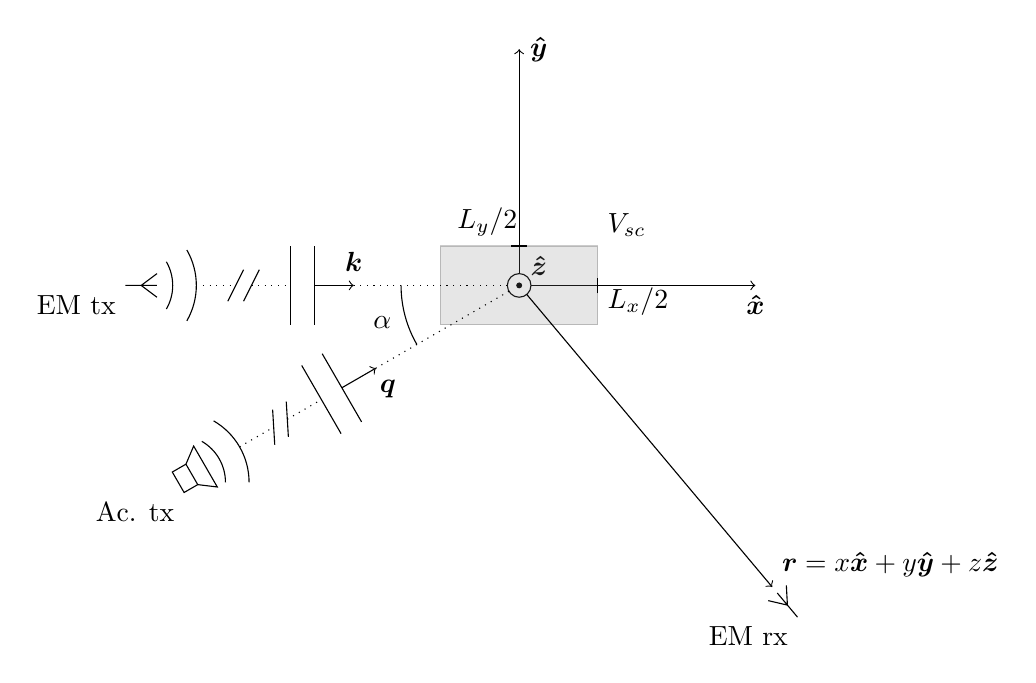
\begin{tikzpicture}
			% Draw coordinate axes
			\draw (0,0) circle(0.15);
			\filldraw[black] circle(0.03);
			\draw[->] (0.15,0) -- (3,0);
			\draw[->] (0,.150) -- (0,3);
			\draw (3,-0.25) node{$\bm{\hat{x}}$} (0.25,3) node{$\bm{\hat{y}}$} (0.25,0.25) node{$\bm{\hat{z}}$};
			
			% Draw scattering cube (or rectangle in this case)
			\draw[fill=gray,opacity=0.2] (-1,-0.5) rectangle(1,0.5);
			\draw (1,-0.1) -- (1,0.1) node[anchor= north west]{$L_{x}/2$} (-0.1,0.5) -- (0.1,0.5) node[anchor= south east]{$L_{y}/2$} (1,0.5) node[anchor=south west]{$V_\mrm{sc}$};
			
			% Draw EM tx and spherical waves
			\draw[shift = {(-5,0)}] (0,0) node[anchor=north east]{EM tx} -- (0.4,0) (0.2,0) -- (0.4,0.15)
			(0.2,0) -- (0.4,-0.15);
			\draw[shift = {(-5,0)}] ([shift={(-30:0.6)}] 0,0) arc(-30:30:0.6) ([shift={(-30:0.9)}] 0,0) arc(-30:30:0.9);
			
			% Draw EM "long distance" lines
			\draw[shift = {(-4.1,0)},dotted] (0,0) -- (0.5,0) (0.7,0) -- (1.2,0);
			\draw[shift = {(-4.1,0)}] (0.4,-0.2) -- (0.6,0.2) (0.6,-0.2) -- (0.8,0.2);
			
			% Draw EM plane waves
			\draw[shift = {(-2.9,0)}] (0,-0.5) -- (0,0.5) (0.3,-0.5) -- (0.3,0.5);
			\draw[shift = {(-2.6,0)}, ->] (0,0) -- (0.5,0);
			\draw[shift = {(-2.6,0)}] (0.5,0.3) node{$\bm{k}$};
			\draw[dotted] (-0.15,0) -- (-2.1,0);
			
			% Draw Ac. tx and spherical waves
			\draw[shift = {(210:5)}, rotate = 30] (0,-0.15) node[anchor=north east]{Ac. tx} rectangle (0.2,0.15) -- (0.4,0.3) -- (0.4,-0.3) -- (0.2,-0.15);
			\draw[shift = {(210:5)}, rotate = 30] ([shift={(-30:0.6)}] 0,0) arc(-30:30:0.6) ([shift={(-30:0.9)}] 0,0) arc(-30:30:0.9);
			
			% Draw Ac. "long distance" lines
			\draw[shift = {(210:4.1)}, rotate = 30,dotted] (0,0) -- (0.5,0) (0.7,0) -- (1.2,0);
			\draw[shift = {(210:4.1)}, rotate = 30] (0.4,-0.2) -- (0.6,0.2) (0.6,-0.2) -- (0.8,0.2);
			
			% Draw Ac. plane waves
			\draw[shift = {(210:2.9)}, rotate = 30] (0,-0.5) -- (0,0.5) (0.3,-0.5) -- (0.3,0.5);
			\draw[shift = {(210:2.6)}, rotate = 30, ->] (0,0) -- (0.5,0);
			\draw[shift = {(210:2.6)}, rotate = 30] (0.5,-0.3) node{$\bm{q}$};
			\draw[rotate = 30, dotted] (-0.15,0) -- (-2.1,0);
			
			% Draw angle alpha
			\draw ([shift={(180:1.5)}] 0,0) arc(180:210:1.5) (195:1.8) node{$\alpha$};
			
			% Draw line towards receiver
			\draw[->] (310:0.15) -- (310:5) node[anchor=south west]{$\bm{r} = x\bm{\hat{x}} + y\bm{\hat{y}} + z\bm{\hat{z}}$};
			
			% Draw EM rx
			\draw[shift = {(310:5.5)}, rotate = 130] (0,0) node[anchor=north east]{EM rx} -- (0.4,0) (0.2,0) -- (0.4,0.15) (0.2,0) -- (0.4,-0.15);
		\end{tikzpicture}
		}
		
	Plane waves in simple interaction region
	\end{frame}
	
	\begin{frame}{Theory}{Plane wave solution}
		\begin{itemize}
			\item Scattering integral solution
			\small
			\begin{equation*}
				\bm{E}_\mrm{sc} (\bm{r},t) = \bm{E}_{\mrm{i}0} \left( E_\mrm{A}^+ (\bm{r},t) + E_\mrm{A}^- (\bm{r},t) \right)
			\end{equation*}
			\begin{equation*}
				E_\mrm{A}^\pm (\bm{r},t) = \frac{\varepsilon_\mrm{r}k^2 \eu^{\iu kr} \mathfrak{p} p_0}{8\pi r K} L_{x} L_{y} L_{z} e^{\mp \iu \Omega t} \Phi^\pm (\theta,\phi)
			\end{equation*}
			\begin{equation*}
			\begin{split}
				\Phi^\pm(\theta,\phi) =& \text{sinc} \left( \frac{L_{x}}{2\pi} \left( k - k\sin{\theta}\cos{\phi} \pm q\cos{\alpha} \right) \right) \\
				\cdot& \text{sinc} \left( \frac{L_{y}}{2\pi} \left( -k\sin{\theta}\sin{\phi} \pm q\sin{\alpha} \right) \right)
				\cdot \text{sinc} \left( -\frac{L_{z}}{2\pi} k\cos{\theta} \right)
			\end{split}
			\end{equation*}
			\pause
			\normalsize
			\item Frequency of scattered wave shifted by $\pm \Omega$
			\item Phase matching given by Bragg condition
		\end{itemize}
	\end{frame}

	\section{Numerical Simulation}
	
	\begin{frame}{Numerical Simulation}{Preparations}
		\begin{itemize}
			\item COMSOL Multiphysics
			\pause
			\item Circular geometry in 2D
			\item Boundary condition simulating open boundary
			\pause
			\item Frequencies selected for phase matching at $\alpha = 40^\circ$ (-) and $\alpha = 140^\circ$ (+)
			\pause
			\item Studies:
			\begin{itemize}
				\item Sweep of angle $\alpha$
				\item Defect with electric contrast
				\item Defect with acoustic contrast
			\end{itemize}
		\end{itemize}
	\end{frame}
	
	\begin{frame}{Numerical Simulation}{$\alpha = 40^\circ$, Frequency shift $-\Omega$}
		\begin{figure}
			\centering
			\begin{subfigure}{0.5\textheight}
				\includegraphics[width=\textwidth]{../../Text/Report/fig/anglesweep(-)_nolabel_p.png}
			\end{subfigure}
			\begin{subfigure}{0.5\textheight}
				\includegraphics[width=\textwidth]{../../Text/Report/fig/anglesweep(-)_nolabel_Ez.png}
			\end{subfigure}
			\begin{subfigure}{0.5\textheight}
				\includegraphics[width=\textwidth]{../../Text/Report/fig/anglesweep(-)_nolabel_diff.png}
			\end{subfigure}
			\begin{subfigure}{0.5\textheight}
				\includegraphics[width=\textwidth]{../../Text/Report/fig/anglesweep(-)_nolabel_power.png}
			\end{subfigure}
		\end{figure}
	\end{frame}
	
	\begin{frame}{Numerical Simulation}{$\alpha = 140^\circ$, Frequency shift $+\Omega$}
		\begin{figure}
			\centering
			\begin{subfigure}{0.5\textheight}
				\includegraphics[width=\textwidth]{../../Text/Report/fig/anglesweep(+)_nolabel_p.png}
			\end{subfigure}
			\begin{subfigure}{0.5\textheight}
				\includegraphics[width=\textwidth]{../../Text/Report/fig/anglesweep(+)_nolabel_Ez.png}
			\end{subfigure}
			\begin{subfigure}{0.5\textheight}
				\includegraphics[width=\textwidth]{../../Text/Report/fig/anglesweep(+)_nolabel_diff.png}
			\end{subfigure}
			\begin{subfigure}{0.5\textheight}
				\includegraphics[width=\textwidth]{../../Text/Report/fig/anglesweep(+)_nolabel_power.png}
			\end{subfigure}
		\end{figure}
	\end{frame}
	
	\begin{frame}{Numerical Simulation}{Sweep of angle $\alpha$, total scattered power}
		\begin{columns}
			\begin{column}{0.5\textwidth}
				\begin{figure}
					\centering
					\resizebox{\textwidth}{!}{%% Creator: Matplotlib, PGF backend
%%
%% To include the figure in your LaTeX document, write
%%   \input{<filename>.pgf}
%%
%% Make sure the required packages are loaded in your preamble
%%   \usepackage{pgf}
%%
%% Figures using additional raster images can only be included by \input if
%% they are in the same directory as the main LaTeX file. For loading figures
%% from other directories you can use the `import` package
%%   \usepackage{import}
%% and then include the figures with
%%   \import{<path to file>}{<filename>.pgf}
%%
%% Matplotlib used the following preamble
%%   \usepackage{fontspec}
%%   \setmainfont{DejaVu Serif}
%%   \setsansfont{DejaVu Sans}
%%   \setmonofont{DejaVu Sans Mono}
%%
\begingroup%
\makeatletter%
\begin{pgfpicture}%
\pgfpathrectangle{\pgfpointorigin}{\pgfqpoint{6.400000in}{4.800000in}}%
\pgfusepath{use as bounding box, clip}%
\begin{pgfscope}%
\pgfsetbuttcap%
\pgfsetmiterjoin%
\definecolor{currentfill}{rgb}{1.000000,1.000000,1.000000}%
\pgfsetfillcolor{currentfill}%
\pgfsetlinewidth{0.000000pt}%
\definecolor{currentstroke}{rgb}{1.000000,1.000000,1.000000}%
\pgfsetstrokecolor{currentstroke}%
\pgfsetdash{}{0pt}%
\pgfpathmoveto{\pgfqpoint{0.000000in}{0.000000in}}%
\pgfpathlineto{\pgfqpoint{6.400000in}{0.000000in}}%
\pgfpathlineto{\pgfqpoint{6.400000in}{4.800000in}}%
\pgfpathlineto{\pgfqpoint{0.000000in}{4.800000in}}%
\pgfpathclose%
\pgfusepath{fill}%
\end{pgfscope}%
\begin{pgfscope}%
\pgfsetbuttcap%
\pgfsetmiterjoin%
\definecolor{currentfill}{rgb}{1.000000,1.000000,1.000000}%
\pgfsetfillcolor{currentfill}%
\pgfsetlinewidth{0.000000pt}%
\definecolor{currentstroke}{rgb}{0.000000,0.000000,0.000000}%
\pgfsetstrokecolor{currentstroke}%
\pgfsetstrokeopacity{0.000000}%
\pgfsetdash{}{0pt}%
\pgfpathmoveto{\pgfqpoint{0.800000in}{0.528000in}}%
\pgfpathlineto{\pgfqpoint{5.760000in}{0.528000in}}%
\pgfpathlineto{\pgfqpoint{5.760000in}{4.224000in}}%
\pgfpathlineto{\pgfqpoint{0.800000in}{4.224000in}}%
\pgfpathclose%
\pgfusepath{fill}%
\end{pgfscope}%
\begin{pgfscope}%
\pgfpathrectangle{\pgfqpoint{0.800000in}{0.528000in}}{\pgfqpoint{4.960000in}{3.696000in}} %
\pgfusepath{clip}%
\pgfsetrectcap%
\pgfsetroundjoin%
\pgfsetlinewidth{0.803000pt}%
\definecolor{currentstroke}{rgb}{0.690196,0.690196,0.690196}%
\pgfsetstrokecolor{currentstroke}%
\pgfsetdash{}{0pt}%
\pgfpathmoveto{\pgfqpoint{0.800000in}{0.528000in}}%
\pgfpathlineto{\pgfqpoint{0.800000in}{4.224000in}}%
\pgfusepath{stroke}%
\end{pgfscope}%
\begin{pgfscope}%
\pgfsetbuttcap%
\pgfsetroundjoin%
\definecolor{currentfill}{rgb}{0.000000,0.000000,0.000000}%
\pgfsetfillcolor{currentfill}%
\pgfsetlinewidth{0.803000pt}%
\definecolor{currentstroke}{rgb}{0.000000,0.000000,0.000000}%
\pgfsetstrokecolor{currentstroke}%
\pgfsetdash{}{0pt}%
\pgfsys@defobject{currentmarker}{\pgfqpoint{0.000000in}{-0.048611in}}{\pgfqpoint{0.000000in}{0.000000in}}{%
\pgfpathmoveto{\pgfqpoint{0.000000in}{0.000000in}}%
\pgfpathlineto{\pgfqpoint{0.000000in}{-0.048611in}}%
\pgfusepath{stroke,fill}%
}%
\begin{pgfscope}%
\pgfsys@transformshift{0.800000in}{0.528000in}%
\pgfsys@useobject{currentmarker}{}%
\end{pgfscope}%
\end{pgfscope}%
\begin{pgfscope}%
\pgftext[x=0.800000in,y=0.430778in,,top]{\sffamily\fontsize{10.000000}{12.000000}\selectfont 34\(\displaystyle ^\circ\)}%
\end{pgfscope}%
\begin{pgfscope}%
\pgfpathrectangle{\pgfqpoint{0.800000in}{0.528000in}}{\pgfqpoint{4.960000in}{3.696000in}} %
\pgfusepath{clip}%
\pgfsetrectcap%
\pgfsetroundjoin%
\pgfsetlinewidth{0.803000pt}%
\definecolor{currentstroke}{rgb}{0.690196,0.690196,0.690196}%
\pgfsetstrokecolor{currentstroke}%
\pgfsetdash{}{0pt}%
\pgfpathmoveto{\pgfqpoint{1.626667in}{0.528000in}}%
\pgfpathlineto{\pgfqpoint{1.626667in}{4.224000in}}%
\pgfusepath{stroke}%
\end{pgfscope}%
\begin{pgfscope}%
\pgfsetbuttcap%
\pgfsetroundjoin%
\definecolor{currentfill}{rgb}{0.000000,0.000000,0.000000}%
\pgfsetfillcolor{currentfill}%
\pgfsetlinewidth{0.803000pt}%
\definecolor{currentstroke}{rgb}{0.000000,0.000000,0.000000}%
\pgfsetstrokecolor{currentstroke}%
\pgfsetdash{}{0pt}%
\pgfsys@defobject{currentmarker}{\pgfqpoint{0.000000in}{-0.048611in}}{\pgfqpoint{0.000000in}{0.000000in}}{%
\pgfpathmoveto{\pgfqpoint{0.000000in}{0.000000in}}%
\pgfpathlineto{\pgfqpoint{0.000000in}{-0.048611in}}%
\pgfusepath{stroke,fill}%
}%
\begin{pgfscope}%
\pgfsys@transformshift{1.626667in}{0.528000in}%
\pgfsys@useobject{currentmarker}{}%
\end{pgfscope}%
\end{pgfscope}%
\begin{pgfscope}%
\pgftext[x=1.626667in,y=0.430778in,,top]{\sffamily\fontsize{10.000000}{12.000000}\selectfont 36\(\displaystyle ^\circ\)}%
\end{pgfscope}%
\begin{pgfscope}%
\pgfpathrectangle{\pgfqpoint{0.800000in}{0.528000in}}{\pgfqpoint{4.960000in}{3.696000in}} %
\pgfusepath{clip}%
\pgfsetrectcap%
\pgfsetroundjoin%
\pgfsetlinewidth{0.803000pt}%
\definecolor{currentstroke}{rgb}{0.690196,0.690196,0.690196}%
\pgfsetstrokecolor{currentstroke}%
\pgfsetdash{}{0pt}%
\pgfpathmoveto{\pgfqpoint{2.453333in}{0.528000in}}%
\pgfpathlineto{\pgfqpoint{2.453333in}{4.224000in}}%
\pgfusepath{stroke}%
\end{pgfscope}%
\begin{pgfscope}%
\pgfsetbuttcap%
\pgfsetroundjoin%
\definecolor{currentfill}{rgb}{0.000000,0.000000,0.000000}%
\pgfsetfillcolor{currentfill}%
\pgfsetlinewidth{0.803000pt}%
\definecolor{currentstroke}{rgb}{0.000000,0.000000,0.000000}%
\pgfsetstrokecolor{currentstroke}%
\pgfsetdash{}{0pt}%
\pgfsys@defobject{currentmarker}{\pgfqpoint{0.000000in}{-0.048611in}}{\pgfqpoint{0.000000in}{0.000000in}}{%
\pgfpathmoveto{\pgfqpoint{0.000000in}{0.000000in}}%
\pgfpathlineto{\pgfqpoint{0.000000in}{-0.048611in}}%
\pgfusepath{stroke,fill}%
}%
\begin{pgfscope}%
\pgfsys@transformshift{2.453333in}{0.528000in}%
\pgfsys@useobject{currentmarker}{}%
\end{pgfscope}%
\end{pgfscope}%
\begin{pgfscope}%
\pgftext[x=2.453333in,y=0.430778in,,top]{\sffamily\fontsize{10.000000}{12.000000}\selectfont 38\(\displaystyle ^\circ\)}%
\end{pgfscope}%
\begin{pgfscope}%
\pgfpathrectangle{\pgfqpoint{0.800000in}{0.528000in}}{\pgfqpoint{4.960000in}{3.696000in}} %
\pgfusepath{clip}%
\pgfsetrectcap%
\pgfsetroundjoin%
\pgfsetlinewidth{0.803000pt}%
\definecolor{currentstroke}{rgb}{0.690196,0.690196,0.690196}%
\pgfsetstrokecolor{currentstroke}%
\pgfsetdash{}{0pt}%
\pgfpathmoveto{\pgfqpoint{3.280000in}{0.528000in}}%
\pgfpathlineto{\pgfqpoint{3.280000in}{4.224000in}}%
\pgfusepath{stroke}%
\end{pgfscope}%
\begin{pgfscope}%
\pgfsetbuttcap%
\pgfsetroundjoin%
\definecolor{currentfill}{rgb}{0.000000,0.000000,0.000000}%
\pgfsetfillcolor{currentfill}%
\pgfsetlinewidth{0.803000pt}%
\definecolor{currentstroke}{rgb}{0.000000,0.000000,0.000000}%
\pgfsetstrokecolor{currentstroke}%
\pgfsetdash{}{0pt}%
\pgfsys@defobject{currentmarker}{\pgfqpoint{0.000000in}{-0.048611in}}{\pgfqpoint{0.000000in}{0.000000in}}{%
\pgfpathmoveto{\pgfqpoint{0.000000in}{0.000000in}}%
\pgfpathlineto{\pgfqpoint{0.000000in}{-0.048611in}}%
\pgfusepath{stroke,fill}%
}%
\begin{pgfscope}%
\pgfsys@transformshift{3.280000in}{0.528000in}%
\pgfsys@useobject{currentmarker}{}%
\end{pgfscope}%
\end{pgfscope}%
\begin{pgfscope}%
\pgftext[x=3.280000in,y=0.430778in,,top]{\sffamily\fontsize{10.000000}{12.000000}\selectfont 40\(\displaystyle ^\circ\)}%
\end{pgfscope}%
\begin{pgfscope}%
\pgfpathrectangle{\pgfqpoint{0.800000in}{0.528000in}}{\pgfqpoint{4.960000in}{3.696000in}} %
\pgfusepath{clip}%
\pgfsetrectcap%
\pgfsetroundjoin%
\pgfsetlinewidth{0.803000pt}%
\definecolor{currentstroke}{rgb}{0.690196,0.690196,0.690196}%
\pgfsetstrokecolor{currentstroke}%
\pgfsetdash{}{0pt}%
\pgfpathmoveto{\pgfqpoint{4.106667in}{0.528000in}}%
\pgfpathlineto{\pgfqpoint{4.106667in}{4.224000in}}%
\pgfusepath{stroke}%
\end{pgfscope}%
\begin{pgfscope}%
\pgfsetbuttcap%
\pgfsetroundjoin%
\definecolor{currentfill}{rgb}{0.000000,0.000000,0.000000}%
\pgfsetfillcolor{currentfill}%
\pgfsetlinewidth{0.803000pt}%
\definecolor{currentstroke}{rgb}{0.000000,0.000000,0.000000}%
\pgfsetstrokecolor{currentstroke}%
\pgfsetdash{}{0pt}%
\pgfsys@defobject{currentmarker}{\pgfqpoint{0.000000in}{-0.048611in}}{\pgfqpoint{0.000000in}{0.000000in}}{%
\pgfpathmoveto{\pgfqpoint{0.000000in}{0.000000in}}%
\pgfpathlineto{\pgfqpoint{0.000000in}{-0.048611in}}%
\pgfusepath{stroke,fill}%
}%
\begin{pgfscope}%
\pgfsys@transformshift{4.106667in}{0.528000in}%
\pgfsys@useobject{currentmarker}{}%
\end{pgfscope}%
\end{pgfscope}%
\begin{pgfscope}%
\pgftext[x=4.106667in,y=0.430778in,,top]{\sffamily\fontsize{10.000000}{12.000000}\selectfont 42\(\displaystyle ^\circ\)}%
\end{pgfscope}%
\begin{pgfscope}%
\pgfpathrectangle{\pgfqpoint{0.800000in}{0.528000in}}{\pgfqpoint{4.960000in}{3.696000in}} %
\pgfusepath{clip}%
\pgfsetrectcap%
\pgfsetroundjoin%
\pgfsetlinewidth{0.803000pt}%
\definecolor{currentstroke}{rgb}{0.690196,0.690196,0.690196}%
\pgfsetstrokecolor{currentstroke}%
\pgfsetdash{}{0pt}%
\pgfpathmoveto{\pgfqpoint{4.933333in}{0.528000in}}%
\pgfpathlineto{\pgfqpoint{4.933333in}{4.224000in}}%
\pgfusepath{stroke}%
\end{pgfscope}%
\begin{pgfscope}%
\pgfsetbuttcap%
\pgfsetroundjoin%
\definecolor{currentfill}{rgb}{0.000000,0.000000,0.000000}%
\pgfsetfillcolor{currentfill}%
\pgfsetlinewidth{0.803000pt}%
\definecolor{currentstroke}{rgb}{0.000000,0.000000,0.000000}%
\pgfsetstrokecolor{currentstroke}%
\pgfsetdash{}{0pt}%
\pgfsys@defobject{currentmarker}{\pgfqpoint{0.000000in}{-0.048611in}}{\pgfqpoint{0.000000in}{0.000000in}}{%
\pgfpathmoveto{\pgfqpoint{0.000000in}{0.000000in}}%
\pgfpathlineto{\pgfqpoint{0.000000in}{-0.048611in}}%
\pgfusepath{stroke,fill}%
}%
\begin{pgfscope}%
\pgfsys@transformshift{4.933333in}{0.528000in}%
\pgfsys@useobject{currentmarker}{}%
\end{pgfscope}%
\end{pgfscope}%
\begin{pgfscope}%
\pgftext[x=4.933333in,y=0.430778in,,top]{\sffamily\fontsize{10.000000}{12.000000}\selectfont 44\(\displaystyle ^\circ\)}%
\end{pgfscope}%
\begin{pgfscope}%
\pgfpathrectangle{\pgfqpoint{0.800000in}{0.528000in}}{\pgfqpoint{4.960000in}{3.696000in}} %
\pgfusepath{clip}%
\pgfsetrectcap%
\pgfsetroundjoin%
\pgfsetlinewidth{0.803000pt}%
\definecolor{currentstroke}{rgb}{0.690196,0.690196,0.690196}%
\pgfsetstrokecolor{currentstroke}%
\pgfsetdash{}{0pt}%
\pgfpathmoveto{\pgfqpoint{5.760000in}{0.528000in}}%
\pgfpathlineto{\pgfqpoint{5.760000in}{4.224000in}}%
\pgfusepath{stroke}%
\end{pgfscope}%
\begin{pgfscope}%
\pgfsetbuttcap%
\pgfsetroundjoin%
\definecolor{currentfill}{rgb}{0.000000,0.000000,0.000000}%
\pgfsetfillcolor{currentfill}%
\pgfsetlinewidth{0.803000pt}%
\definecolor{currentstroke}{rgb}{0.000000,0.000000,0.000000}%
\pgfsetstrokecolor{currentstroke}%
\pgfsetdash{}{0pt}%
\pgfsys@defobject{currentmarker}{\pgfqpoint{0.000000in}{-0.048611in}}{\pgfqpoint{0.000000in}{0.000000in}}{%
\pgfpathmoveto{\pgfqpoint{0.000000in}{0.000000in}}%
\pgfpathlineto{\pgfqpoint{0.000000in}{-0.048611in}}%
\pgfusepath{stroke,fill}%
}%
\begin{pgfscope}%
\pgfsys@transformshift{5.760000in}{0.528000in}%
\pgfsys@useobject{currentmarker}{}%
\end{pgfscope}%
\end{pgfscope}%
\begin{pgfscope}%
\pgftext[x=5.760000in,y=0.430778in,,top]{\sffamily\fontsize{10.000000}{12.000000}\selectfont 46\(\displaystyle ^\circ\)}%
\end{pgfscope}%
\begin{pgfscope}%
\pgftext[x=3.280000in,y=0.240809in,,top]{\sffamily\fontsize{10.000000}{12.000000}\selectfont \(\displaystyle \alpha\)}%
\end{pgfscope}%
\begin{pgfscope}%
\pgfpathrectangle{\pgfqpoint{0.800000in}{0.528000in}}{\pgfqpoint{4.960000in}{3.696000in}} %
\pgfusepath{clip}%
\pgfsetrectcap%
\pgfsetroundjoin%
\pgfsetlinewidth{0.803000pt}%
\definecolor{currentstroke}{rgb}{0.690196,0.690196,0.690196}%
\pgfsetstrokecolor{currentstroke}%
\pgfsetdash{}{0pt}%
\pgfpathmoveto{\pgfqpoint{0.800000in}{1.113586in}}%
\pgfpathlineto{\pgfqpoint{5.760000in}{1.113586in}}%
\pgfusepath{stroke}%
\end{pgfscope}%
\begin{pgfscope}%
\pgfsetbuttcap%
\pgfsetroundjoin%
\definecolor{currentfill}{rgb}{0.000000,0.000000,0.000000}%
\pgfsetfillcolor{currentfill}%
\pgfsetlinewidth{0.803000pt}%
\definecolor{currentstroke}{rgb}{0.000000,0.000000,0.000000}%
\pgfsetstrokecolor{currentstroke}%
\pgfsetdash{}{0pt}%
\pgfsys@defobject{currentmarker}{\pgfqpoint{-0.048611in}{0.000000in}}{\pgfqpoint{0.000000in}{0.000000in}}{%
\pgfpathmoveto{\pgfqpoint{0.000000in}{0.000000in}}%
\pgfpathlineto{\pgfqpoint{-0.048611in}{0.000000in}}%
\pgfusepath{stroke,fill}%
}%
\begin{pgfscope}%
\pgfsys@transformshift{0.800000in}{1.113586in}%
\pgfsys@useobject{currentmarker}{}%
\end{pgfscope}%
\end{pgfscope}%
\begin{pgfscope}%
\pgftext[x=0.475930in,y=1.060825in,left,base]{\sffamily\fontsize{10.000000}{12.000000}\selectfont -92}%
\end{pgfscope}%
\begin{pgfscope}%
\pgfpathrectangle{\pgfqpoint{0.800000in}{0.528000in}}{\pgfqpoint{4.960000in}{3.696000in}} %
\pgfusepath{clip}%
\pgfsetrectcap%
\pgfsetroundjoin%
\pgfsetlinewidth{0.803000pt}%
\definecolor{currentstroke}{rgb}{0.690196,0.690196,0.690196}%
\pgfsetstrokecolor{currentstroke}%
\pgfsetdash{}{0pt}%
\pgfpathmoveto{\pgfqpoint{0.800000in}{1.741828in}}%
\pgfpathlineto{\pgfqpoint{5.760000in}{1.741828in}}%
\pgfusepath{stroke}%
\end{pgfscope}%
\begin{pgfscope}%
\pgfsetbuttcap%
\pgfsetroundjoin%
\definecolor{currentfill}{rgb}{0.000000,0.000000,0.000000}%
\pgfsetfillcolor{currentfill}%
\pgfsetlinewidth{0.803000pt}%
\definecolor{currentstroke}{rgb}{0.000000,0.000000,0.000000}%
\pgfsetstrokecolor{currentstroke}%
\pgfsetdash{}{0pt}%
\pgfsys@defobject{currentmarker}{\pgfqpoint{-0.048611in}{0.000000in}}{\pgfqpoint{0.000000in}{0.000000in}}{%
\pgfpathmoveto{\pgfqpoint{0.000000in}{0.000000in}}%
\pgfpathlineto{\pgfqpoint{-0.048611in}{0.000000in}}%
\pgfusepath{stroke,fill}%
}%
\begin{pgfscope}%
\pgfsys@transformshift{0.800000in}{1.741828in}%
\pgfsys@useobject{currentmarker}{}%
\end{pgfscope}%
\end{pgfscope}%
\begin{pgfscope}%
\pgftext[x=0.475930in,y=1.689066in,left,base]{\sffamily\fontsize{10.000000}{12.000000}\selectfont -90}%
\end{pgfscope}%
\begin{pgfscope}%
\pgfpathrectangle{\pgfqpoint{0.800000in}{0.528000in}}{\pgfqpoint{4.960000in}{3.696000in}} %
\pgfusepath{clip}%
\pgfsetrectcap%
\pgfsetroundjoin%
\pgfsetlinewidth{0.803000pt}%
\definecolor{currentstroke}{rgb}{0.690196,0.690196,0.690196}%
\pgfsetstrokecolor{currentstroke}%
\pgfsetdash{}{0pt}%
\pgfpathmoveto{\pgfqpoint{0.800000in}{2.370070in}}%
\pgfpathlineto{\pgfqpoint{5.760000in}{2.370070in}}%
\pgfusepath{stroke}%
\end{pgfscope}%
\begin{pgfscope}%
\pgfsetbuttcap%
\pgfsetroundjoin%
\definecolor{currentfill}{rgb}{0.000000,0.000000,0.000000}%
\pgfsetfillcolor{currentfill}%
\pgfsetlinewidth{0.803000pt}%
\definecolor{currentstroke}{rgb}{0.000000,0.000000,0.000000}%
\pgfsetstrokecolor{currentstroke}%
\pgfsetdash{}{0pt}%
\pgfsys@defobject{currentmarker}{\pgfqpoint{-0.048611in}{0.000000in}}{\pgfqpoint{0.000000in}{0.000000in}}{%
\pgfpathmoveto{\pgfqpoint{0.000000in}{0.000000in}}%
\pgfpathlineto{\pgfqpoint{-0.048611in}{0.000000in}}%
\pgfusepath{stroke,fill}%
}%
\begin{pgfscope}%
\pgfsys@transformshift{0.800000in}{2.370070in}%
\pgfsys@useobject{currentmarker}{}%
\end{pgfscope}%
\end{pgfscope}%
\begin{pgfscope}%
\pgftext[x=0.475930in,y=2.317308in,left,base]{\sffamily\fontsize{10.000000}{12.000000}\selectfont -88}%
\end{pgfscope}%
\begin{pgfscope}%
\pgfpathrectangle{\pgfqpoint{0.800000in}{0.528000in}}{\pgfqpoint{4.960000in}{3.696000in}} %
\pgfusepath{clip}%
\pgfsetrectcap%
\pgfsetroundjoin%
\pgfsetlinewidth{0.803000pt}%
\definecolor{currentstroke}{rgb}{0.690196,0.690196,0.690196}%
\pgfsetstrokecolor{currentstroke}%
\pgfsetdash{}{0pt}%
\pgfpathmoveto{\pgfqpoint{0.800000in}{2.998311in}}%
\pgfpathlineto{\pgfqpoint{5.760000in}{2.998311in}}%
\pgfusepath{stroke}%
\end{pgfscope}%
\begin{pgfscope}%
\pgfsetbuttcap%
\pgfsetroundjoin%
\definecolor{currentfill}{rgb}{0.000000,0.000000,0.000000}%
\pgfsetfillcolor{currentfill}%
\pgfsetlinewidth{0.803000pt}%
\definecolor{currentstroke}{rgb}{0.000000,0.000000,0.000000}%
\pgfsetstrokecolor{currentstroke}%
\pgfsetdash{}{0pt}%
\pgfsys@defobject{currentmarker}{\pgfqpoint{-0.048611in}{0.000000in}}{\pgfqpoint{0.000000in}{0.000000in}}{%
\pgfpathmoveto{\pgfqpoint{0.000000in}{0.000000in}}%
\pgfpathlineto{\pgfqpoint{-0.048611in}{0.000000in}}%
\pgfusepath{stroke,fill}%
}%
\begin{pgfscope}%
\pgfsys@transformshift{0.800000in}{2.998311in}%
\pgfsys@useobject{currentmarker}{}%
\end{pgfscope}%
\end{pgfscope}%
\begin{pgfscope}%
\pgftext[x=0.475930in,y=2.945550in,left,base]{\sffamily\fontsize{10.000000}{12.000000}\selectfont -86}%
\end{pgfscope}%
\begin{pgfscope}%
\pgfpathrectangle{\pgfqpoint{0.800000in}{0.528000in}}{\pgfqpoint{4.960000in}{3.696000in}} %
\pgfusepath{clip}%
\pgfsetrectcap%
\pgfsetroundjoin%
\pgfsetlinewidth{0.803000pt}%
\definecolor{currentstroke}{rgb}{0.690196,0.690196,0.690196}%
\pgfsetstrokecolor{currentstroke}%
\pgfsetdash{}{0pt}%
\pgfpathmoveto{\pgfqpoint{0.800000in}{3.626553in}}%
\pgfpathlineto{\pgfqpoint{5.760000in}{3.626553in}}%
\pgfusepath{stroke}%
\end{pgfscope}%
\begin{pgfscope}%
\pgfsetbuttcap%
\pgfsetroundjoin%
\definecolor{currentfill}{rgb}{0.000000,0.000000,0.000000}%
\pgfsetfillcolor{currentfill}%
\pgfsetlinewidth{0.803000pt}%
\definecolor{currentstroke}{rgb}{0.000000,0.000000,0.000000}%
\pgfsetstrokecolor{currentstroke}%
\pgfsetdash{}{0pt}%
\pgfsys@defobject{currentmarker}{\pgfqpoint{-0.048611in}{0.000000in}}{\pgfqpoint{0.000000in}{0.000000in}}{%
\pgfpathmoveto{\pgfqpoint{0.000000in}{0.000000in}}%
\pgfpathlineto{\pgfqpoint{-0.048611in}{0.000000in}}%
\pgfusepath{stroke,fill}%
}%
\begin{pgfscope}%
\pgfsys@transformshift{0.800000in}{3.626553in}%
\pgfsys@useobject{currentmarker}{}%
\end{pgfscope}%
\end{pgfscope}%
\begin{pgfscope}%
\pgftext[x=0.475930in,y=3.573791in,left,base]{\sffamily\fontsize{10.000000}{12.000000}\selectfont -84}%
\end{pgfscope}%
\begin{pgfscope}%
\pgftext[x=0.420375in,y=2.376000in,,bottom,rotate=90.000000]{\sffamily\fontsize{10.000000}{12.000000}\selectfont \(\displaystyle P_\mathrm{sc}\) [dBm]}%
\end{pgfscope}%
\begin{pgfscope}%
\pgfpathrectangle{\pgfqpoint{0.800000in}{0.528000in}}{\pgfqpoint{4.960000in}{3.696000in}} %
\pgfusepath{clip}%
\pgfsetrectcap%
\pgfsetroundjoin%
\pgfsetlinewidth{1.505625pt}%
\definecolor{currentstroke}{rgb}{0.121569,0.466667,0.705882}%
\pgfsetstrokecolor{currentstroke}%
\pgfsetdash{}{0pt}%
\pgfpathmoveto{\pgfqpoint{1.213333in}{3.661797in}}%
\pgfpathlineto{\pgfqpoint{1.626667in}{3.803815in}}%
\pgfpathlineto{\pgfqpoint{2.040000in}{3.914394in}}%
\pgfpathlineto{\pgfqpoint{2.453333in}{3.992912in}}%
\pgfpathlineto{\pgfqpoint{2.866667in}{4.040345in}}%
\pgfpathlineto{\pgfqpoint{3.280000in}{4.056000in}}%
\pgfpathlineto{\pgfqpoint{3.693333in}{4.039946in}}%
\pgfpathlineto{\pgfqpoint{4.106667in}{3.992275in}}%
\pgfpathlineto{\pgfqpoint{4.520000in}{3.913371in}}%
\pgfpathlineto{\pgfqpoint{4.933333in}{3.802894in}}%
\pgfpathlineto{\pgfqpoint{5.346667in}{3.661291in}}%
\pgfusepath{stroke}%
\end{pgfscope}%
\begin{pgfscope}%
\pgfpathrectangle{\pgfqpoint{0.800000in}{0.528000in}}{\pgfqpoint{4.960000in}{3.696000in}} %
\pgfusepath{clip}%
\pgfsetbuttcap%
\pgfsetroundjoin%
\definecolor{currentfill}{rgb}{0.121569,0.466667,0.705882}%
\pgfsetfillcolor{currentfill}%
\pgfsetlinewidth{1.003750pt}%
\definecolor{currentstroke}{rgb}{0.121569,0.466667,0.705882}%
\pgfsetstrokecolor{currentstroke}%
\pgfsetdash{}{0pt}%
\pgfsys@defobject{currentmarker}{\pgfqpoint{-0.020833in}{-0.020833in}}{\pgfqpoint{0.020833in}{0.020833in}}{%
\pgfpathmoveto{\pgfqpoint{0.000000in}{-0.020833in}}%
\pgfpathcurveto{\pgfqpoint{0.005525in}{-0.020833in}}{\pgfqpoint{0.010825in}{-0.018638in}}{\pgfqpoint{0.014731in}{-0.014731in}}%
\pgfpathcurveto{\pgfqpoint{0.018638in}{-0.010825in}}{\pgfqpoint{0.020833in}{-0.005525in}}{\pgfqpoint{0.020833in}{0.000000in}}%
\pgfpathcurveto{\pgfqpoint{0.020833in}{0.005525in}}{\pgfqpoint{0.018638in}{0.010825in}}{\pgfqpoint{0.014731in}{0.014731in}}%
\pgfpathcurveto{\pgfqpoint{0.010825in}{0.018638in}}{\pgfqpoint{0.005525in}{0.020833in}}{\pgfqpoint{0.000000in}{0.020833in}}%
\pgfpathcurveto{\pgfqpoint{-0.005525in}{0.020833in}}{\pgfqpoint{-0.010825in}{0.018638in}}{\pgfqpoint{-0.014731in}{0.014731in}}%
\pgfpathcurveto{\pgfqpoint{-0.018638in}{0.010825in}}{\pgfqpoint{-0.020833in}{0.005525in}}{\pgfqpoint{-0.020833in}{0.000000in}}%
\pgfpathcurveto{\pgfqpoint{-0.020833in}{-0.005525in}}{\pgfqpoint{-0.018638in}{-0.010825in}}{\pgfqpoint{-0.014731in}{-0.014731in}}%
\pgfpathcurveto{\pgfqpoint{-0.010825in}{-0.018638in}}{\pgfqpoint{-0.005525in}{-0.020833in}}{\pgfqpoint{0.000000in}{-0.020833in}}%
\pgfpathclose%
\pgfusepath{stroke,fill}%
}%
\begin{pgfscope}%
\pgfsys@transformshift{1.213333in}{3.661797in}%
\pgfsys@useobject{currentmarker}{}%
\end{pgfscope}%
\begin{pgfscope}%
\pgfsys@transformshift{1.626667in}{3.803815in}%
\pgfsys@useobject{currentmarker}{}%
\end{pgfscope}%
\begin{pgfscope}%
\pgfsys@transformshift{2.040000in}{3.914394in}%
\pgfsys@useobject{currentmarker}{}%
\end{pgfscope}%
\begin{pgfscope}%
\pgfsys@transformshift{2.453333in}{3.992912in}%
\pgfsys@useobject{currentmarker}{}%
\end{pgfscope}%
\begin{pgfscope}%
\pgfsys@transformshift{2.866667in}{4.040345in}%
\pgfsys@useobject{currentmarker}{}%
\end{pgfscope}%
\begin{pgfscope}%
\pgfsys@transformshift{3.280000in}{4.056000in}%
\pgfsys@useobject{currentmarker}{}%
\end{pgfscope}%
\begin{pgfscope}%
\pgfsys@transformshift{3.693333in}{4.039946in}%
\pgfsys@useobject{currentmarker}{}%
\end{pgfscope}%
\begin{pgfscope}%
\pgfsys@transformshift{4.106667in}{3.992275in}%
\pgfsys@useobject{currentmarker}{}%
\end{pgfscope}%
\begin{pgfscope}%
\pgfsys@transformshift{4.520000in}{3.913371in}%
\pgfsys@useobject{currentmarker}{}%
\end{pgfscope}%
\begin{pgfscope}%
\pgfsys@transformshift{4.933333in}{3.802894in}%
\pgfsys@useobject{currentmarker}{}%
\end{pgfscope}%
\begin{pgfscope}%
\pgfsys@transformshift{5.346667in}{3.661291in}%
\pgfsys@useobject{currentmarker}{}%
\end{pgfscope}%
\end{pgfscope}%
\begin{pgfscope}%
\pgfpathrectangle{\pgfqpoint{0.800000in}{0.528000in}}{\pgfqpoint{4.960000in}{3.696000in}} %
\pgfusepath{clip}%
\pgfsetbuttcap%
\pgfsetroundjoin%
\pgfsetlinewidth{1.505625pt}%
\definecolor{currentstroke}{rgb}{1.000000,0.498039,0.054902}%
\pgfsetstrokecolor{currentstroke}%
\pgfsetdash{{5.550000pt}{2.400000pt}}{0.000000pt}%
\pgfpathmoveto{\pgfqpoint{1.213333in}{1.390601in}}%
\pgfpathlineto{\pgfqpoint{1.254667in}{1.477945in}}%
\pgfpathlineto{\pgfqpoint{1.296000in}{1.563755in}}%
\pgfpathlineto{\pgfqpoint{1.337333in}{1.647926in}}%
\pgfpathlineto{\pgfqpoint{1.378667in}{1.730369in}}%
\pgfpathlineto{\pgfqpoint{1.420000in}{1.811014in}}%
\pgfpathlineto{\pgfqpoint{1.461333in}{1.889804in}}%
\pgfpathlineto{\pgfqpoint{1.502667in}{1.966695in}}%
\pgfpathlineto{\pgfqpoint{1.544000in}{2.041652in}}%
\pgfpathlineto{\pgfqpoint{1.585333in}{2.114651in}}%
\pgfpathlineto{\pgfqpoint{1.626667in}{2.185675in}}%
\pgfpathlineto{\pgfqpoint{1.668000in}{2.254714in}}%
\pgfpathlineto{\pgfqpoint{1.709333in}{2.321762in}}%
\pgfpathlineto{\pgfqpoint{1.750667in}{2.386817in}}%
\pgfpathlineto{\pgfqpoint{1.792000in}{2.449884in}}%
\pgfpathlineto{\pgfqpoint{1.833333in}{2.510967in}}%
\pgfpathlineto{\pgfqpoint{1.874667in}{2.570075in}}%
\pgfpathlineto{\pgfqpoint{1.916000in}{2.627218in}}%
\pgfpathlineto{\pgfqpoint{1.957333in}{2.682408in}}%
\pgfpathlineto{\pgfqpoint{1.998667in}{2.735658in}}%
\pgfpathlineto{\pgfqpoint{2.040000in}{2.786981in}}%
\pgfpathlineto{\pgfqpoint{2.081333in}{2.836393in}}%
\pgfpathlineto{\pgfqpoint{2.122667in}{2.883908in}}%
\pgfpathlineto{\pgfqpoint{2.164000in}{2.929540in}}%
\pgfpathlineto{\pgfqpoint{2.205333in}{2.973306in}}%
\pgfpathlineto{\pgfqpoint{2.246667in}{3.015219in}}%
\pgfpathlineto{\pgfqpoint{2.288000in}{3.055295in}}%
\pgfpathlineto{\pgfqpoint{2.329333in}{3.093547in}}%
\pgfpathlineto{\pgfqpoint{2.370667in}{3.129990in}}%
\pgfpathlineto{\pgfqpoint{2.412000in}{3.164638in}}%
\pgfpathlineto{\pgfqpoint{2.453333in}{3.197502in}}%
\pgfpathlineto{\pgfqpoint{2.494667in}{3.228595in}}%
\pgfpathlineto{\pgfqpoint{2.536000in}{3.257930in}}%
\pgfpathlineto{\pgfqpoint{2.577333in}{3.285516in}}%
\pgfpathlineto{\pgfqpoint{2.618667in}{3.311364in}}%
\pgfpathlineto{\pgfqpoint{2.660000in}{3.335484in}}%
\pgfpathlineto{\pgfqpoint{2.701333in}{3.357884in}}%
\pgfpathlineto{\pgfqpoint{2.742667in}{3.378572in}}%
\pgfpathlineto{\pgfqpoint{2.784000in}{3.397555in}}%
\pgfpathlineto{\pgfqpoint{2.825333in}{3.414840in}}%
\pgfpathlineto{\pgfqpoint{2.866667in}{3.430432in}}%
\pgfpathlineto{\pgfqpoint{2.908000in}{3.444335in}}%
\pgfpathlineto{\pgfqpoint{2.949333in}{3.456554in}}%
\pgfpathlineto{\pgfqpoint{2.990667in}{3.467091in}}%
\pgfpathlineto{\pgfqpoint{3.032000in}{3.475948in}}%
\pgfpathlineto{\pgfqpoint{3.073333in}{3.483127in}}%
\pgfpathlineto{\pgfqpoint{3.114667in}{3.488627in}}%
\pgfpathlineto{\pgfqpoint{3.156000in}{3.492447in}}%
\pgfpathlineto{\pgfqpoint{3.197333in}{3.494587in}}%
\pgfpathlineto{\pgfqpoint{3.238667in}{3.495043in}}%
\pgfpathlineto{\pgfqpoint{3.280000in}{3.493812in}}%
\pgfpathlineto{\pgfqpoint{3.321333in}{3.490889in}}%
\pgfpathlineto{\pgfqpoint{3.362667in}{3.486268in}}%
\pgfpathlineto{\pgfqpoint{3.404000in}{3.479943in}}%
\pgfpathlineto{\pgfqpoint{3.445333in}{3.471905in}}%
\pgfpathlineto{\pgfqpoint{3.486667in}{3.462146in}}%
\pgfpathlineto{\pgfqpoint{3.528000in}{3.450657in}}%
\pgfpathlineto{\pgfqpoint{3.569333in}{3.437424in}}%
\pgfpathlineto{\pgfqpoint{3.610667in}{3.422437in}}%
\pgfpathlineto{\pgfqpoint{3.652000in}{3.405681in}}%
\pgfpathlineto{\pgfqpoint{3.693333in}{3.387141in}}%
\pgfpathlineto{\pgfqpoint{3.734667in}{3.366801in}}%
\pgfpathlineto{\pgfqpoint{3.776000in}{3.344643in}}%
\pgfpathlineto{\pgfqpoint{3.817333in}{3.320647in}}%
\pgfpathlineto{\pgfqpoint{3.858667in}{3.294793in}}%
\pgfpathlineto{\pgfqpoint{3.900000in}{3.267057in}}%
\pgfpathlineto{\pgfqpoint{3.941333in}{3.237415in}}%
\pgfpathlineto{\pgfqpoint{3.982667in}{3.205841in}}%
\pgfpathlineto{\pgfqpoint{4.024000in}{3.172306in}}%
\pgfpathlineto{\pgfqpoint{4.065333in}{3.136780in}}%
\pgfpathlineto{\pgfqpoint{4.106667in}{3.099231in}}%
\pgfpathlineto{\pgfqpoint{4.148000in}{3.059622in}}%
\pgfpathlineto{\pgfqpoint{4.189333in}{3.017917in}}%
\pgfpathlineto{\pgfqpoint{4.230667in}{2.974075in}}%
\pgfpathlineto{\pgfqpoint{4.272000in}{2.928053in}}%
\pgfpathlineto{\pgfqpoint{4.313333in}{2.879803in}}%
\pgfpathlineto{\pgfqpoint{4.354667in}{2.829276in}}%
\pgfpathlineto{\pgfqpoint{4.396000in}{2.776418in}}%
\pgfpathlineto{\pgfqpoint{4.437333in}{2.721172in}}%
\pgfpathlineto{\pgfqpoint{4.478667in}{2.663475in}}%
\pgfpathlineto{\pgfqpoint{4.520000in}{2.603260in}}%
\pgfpathlineto{\pgfqpoint{4.561333in}{2.540456in}}%
\pgfpathlineto{\pgfqpoint{4.602667in}{2.474984in}}%
\pgfpathlineto{\pgfqpoint{4.644000in}{2.406761in}}%
\pgfpathlineto{\pgfqpoint{4.685333in}{2.335695in}}%
\pgfpathlineto{\pgfqpoint{4.726667in}{2.261689in}}%
\pgfpathlineto{\pgfqpoint{4.768000in}{2.184636in}}%
\pgfpathlineto{\pgfqpoint{4.809333in}{2.104421in}}%
\pgfpathlineto{\pgfqpoint{4.850667in}{2.020917in}}%
\pgfpathlineto{\pgfqpoint{4.892000in}{1.933988in}}%
\pgfpathlineto{\pgfqpoint{4.933333in}{1.843484in}}%
\pgfpathlineto{\pgfqpoint{4.974667in}{1.749240in}}%
\pgfpathlineto{\pgfqpoint{5.016000in}{1.651078in}}%
\pgfpathlineto{\pgfqpoint{5.057333in}{1.548800in}}%
\pgfpathlineto{\pgfqpoint{5.098667in}{1.442188in}}%
\pgfpathlineto{\pgfqpoint{5.140000in}{1.331002in}}%
\pgfpathlineto{\pgfqpoint{5.181333in}{1.214975in}}%
\pgfpathlineto{\pgfqpoint{5.222667in}{1.093812in}}%
\pgfpathlineto{\pgfqpoint{5.264000in}{0.967182in}}%
\pgfpathlineto{\pgfqpoint{5.305333in}{0.834716in}}%
\pgfpathlineto{\pgfqpoint{5.346667in}{0.696000in}}%
\pgfusepath{stroke}%
\end{pgfscope}%
\begin{pgfscope}%
\pgfpathrectangle{\pgfqpoint{0.800000in}{0.528000in}}{\pgfqpoint{4.960000in}{3.696000in}} %
\pgfusepath{clip}%
\pgfsetbuttcap%
\pgfsetroundjoin%
\pgfsetlinewidth{1.505625pt}%
\definecolor{currentstroke}{rgb}{0.172549,0.627451,0.172549}%
\pgfsetstrokecolor{currentstroke}%
\pgfsetdash{{1.500000pt}{2.475000pt}}{0.000000pt}%
\pgfpathmoveto{\pgfqpoint{1.213333in}{2.516210in}}%
\pgfpathlineto{\pgfqpoint{1.254667in}{2.563771in}}%
\pgfpathlineto{\pgfqpoint{1.296000in}{2.610483in}}%
\pgfpathlineto{\pgfqpoint{1.337333in}{2.656324in}}%
\pgfpathlineto{\pgfqpoint{1.378667in}{2.701270in}}%
\pgfpathlineto{\pgfqpoint{1.420000in}{2.745301in}}%
\pgfpathlineto{\pgfqpoint{1.461333in}{2.788402in}}%
\pgfpathlineto{\pgfqpoint{1.502667in}{2.830554in}}%
\pgfpathlineto{\pgfqpoint{1.544000in}{2.871745in}}%
\pgfpathlineto{\pgfqpoint{1.585333in}{2.911962in}}%
\pgfpathlineto{\pgfqpoint{1.626667in}{2.951193in}}%
\pgfpathlineto{\pgfqpoint{1.668000in}{2.989430in}}%
\pgfpathlineto{\pgfqpoint{1.709333in}{3.026662in}}%
\pgfpathlineto{\pgfqpoint{1.750667in}{3.062883in}}%
\pgfpathlineto{\pgfqpoint{1.792000in}{3.098086in}}%
\pgfpathlineto{\pgfqpoint{1.833333in}{3.132265in}}%
\pgfpathlineto{\pgfqpoint{1.874667in}{3.165416in}}%
\pgfpathlineto{\pgfqpoint{1.916000in}{3.197535in}}%
\pgfpathlineto{\pgfqpoint{1.957333in}{3.228618in}}%
\pgfpathlineto{\pgfqpoint{1.998667in}{3.258663in}}%
\pgfpathlineto{\pgfqpoint{2.040000in}{3.287667in}}%
\pgfpathlineto{\pgfqpoint{2.081333in}{3.315628in}}%
\pgfpathlineto{\pgfqpoint{2.122667in}{3.342545in}}%
\pgfpathlineto{\pgfqpoint{2.164000in}{3.368418in}}%
\pgfpathlineto{\pgfqpoint{2.205333in}{3.393245in}}%
\pgfpathlineto{\pgfqpoint{2.246667in}{3.417026in}}%
\pgfpathlineto{\pgfqpoint{2.288000in}{3.439761in}}%
\pgfpathlineto{\pgfqpoint{2.329333in}{3.461450in}}%
\pgfpathlineto{\pgfqpoint{2.370667in}{3.482093in}}%
\pgfpathlineto{\pgfqpoint{2.412000in}{3.501692in}}%
\pgfpathlineto{\pgfqpoint{2.453333in}{3.520245in}}%
\pgfpathlineto{\pgfqpoint{2.494667in}{3.537755in}}%
\pgfpathlineto{\pgfqpoint{2.536000in}{3.554221in}}%
\pgfpathlineto{\pgfqpoint{2.577333in}{3.569645in}}%
\pgfpathlineto{\pgfqpoint{2.618667in}{3.584027in}}%
\pgfpathlineto{\pgfqpoint{2.660000in}{3.597368in}}%
\pgfpathlineto{\pgfqpoint{2.701333in}{3.609668in}}%
\pgfpathlineto{\pgfqpoint{2.742667in}{3.620929in}}%
\pgfpathlineto{\pgfqpoint{2.784000in}{3.631151in}}%
\pgfpathlineto{\pgfqpoint{2.825333in}{3.640335in}}%
\pgfpathlineto{\pgfqpoint{2.866667in}{3.648481in}}%
\pgfpathlineto{\pgfqpoint{2.908000in}{3.655591in}}%
\pgfpathlineto{\pgfqpoint{2.949333in}{3.661663in}}%
\pgfpathlineto{\pgfqpoint{2.990667in}{3.666700in}}%
\pgfpathlineto{\pgfqpoint{3.032000in}{3.670700in}}%
\pgfpathlineto{\pgfqpoint{3.073333in}{3.673665in}}%
\pgfpathlineto{\pgfqpoint{3.114667in}{3.675594in}}%
\pgfpathlineto{\pgfqpoint{3.156000in}{3.676488in}}%
\pgfpathlineto{\pgfqpoint{3.197333in}{3.676346in}}%
\pgfpathlineto{\pgfqpoint{3.238667in}{3.675168in}}%
\pgfpathlineto{\pgfqpoint{3.280000in}{3.672954in}}%
\pgfpathlineto{\pgfqpoint{3.321333in}{3.669703in}}%
\pgfpathlineto{\pgfqpoint{3.362667in}{3.665415in}}%
\pgfpathlineto{\pgfqpoint{3.404000in}{3.660090in}}%
\pgfpathlineto{\pgfqpoint{3.445333in}{3.653726in}}%
\pgfpathlineto{\pgfqpoint{3.486667in}{3.646323in}}%
\pgfpathlineto{\pgfqpoint{3.528000in}{3.637880in}}%
\pgfpathlineto{\pgfqpoint{3.569333in}{3.628395in}}%
\pgfpathlineto{\pgfqpoint{3.610667in}{3.617869in}}%
\pgfpathlineto{\pgfqpoint{3.652000in}{3.606300in}}%
\pgfpathlineto{\pgfqpoint{3.693333in}{3.593687in}}%
\pgfpathlineto{\pgfqpoint{3.734667in}{3.580028in}}%
\pgfpathlineto{\pgfqpoint{3.776000in}{3.565323in}}%
\pgfpathlineto{\pgfqpoint{3.817333in}{3.549569in}}%
\pgfpathlineto{\pgfqpoint{3.858667in}{3.532766in}}%
\pgfpathlineto{\pgfqpoint{3.900000in}{3.514913in}}%
\pgfpathlineto{\pgfqpoint{3.941333in}{3.496007in}}%
\pgfpathlineto{\pgfqpoint{3.982667in}{3.476048in}}%
\pgfpathlineto{\pgfqpoint{4.024000in}{3.455034in}}%
\pgfpathlineto{\pgfqpoint{4.065333in}{3.432964in}}%
\pgfpathlineto{\pgfqpoint{4.106667in}{3.409836in}}%
\pgfpathlineto{\pgfqpoint{4.148000in}{3.385650in}}%
\pgfpathlineto{\pgfqpoint{4.189333in}{3.360405in}}%
\pgfpathlineto{\pgfqpoint{4.230667in}{3.334099in}}%
\pgfpathlineto{\pgfqpoint{4.272000in}{3.306732in}}%
\pgfpathlineto{\pgfqpoint{4.313333in}{3.278303in}}%
\pgfpathlineto{\pgfqpoint{4.354667in}{3.248812in}}%
\pgfpathlineto{\pgfqpoint{4.396000in}{3.218259in}}%
\pgfpathlineto{\pgfqpoint{4.437333in}{3.186644in}}%
\pgfpathlineto{\pgfqpoint{4.478667in}{3.153968in}}%
\pgfpathlineto{\pgfqpoint{4.520000in}{3.120231in}}%
\pgfpathlineto{\pgfqpoint{4.561333in}{3.085434in}}%
\pgfpathlineto{\pgfqpoint{4.602667in}{3.049580in}}%
\pgfpathlineto{\pgfqpoint{4.644000in}{3.012672in}}%
\pgfpathlineto{\pgfqpoint{4.685333in}{2.974710in}}%
\pgfpathlineto{\pgfqpoint{4.726667in}{2.935701in}}%
\pgfpathlineto{\pgfqpoint{4.768000in}{2.895647in}}%
\pgfpathlineto{\pgfqpoint{4.809333in}{2.854554in}}%
\pgfpathlineto{\pgfqpoint{4.850667in}{2.812428in}}%
\pgfpathlineto{\pgfqpoint{4.892000in}{2.769276in}}%
\pgfpathlineto{\pgfqpoint{4.933333in}{2.725107in}}%
\pgfpathlineto{\pgfqpoint{4.974667in}{2.679930in}}%
\pgfpathlineto{\pgfqpoint{5.016000in}{2.633756in}}%
\pgfpathlineto{\pgfqpoint{5.057333in}{2.586598in}}%
\pgfpathlineto{\pgfqpoint{5.098667in}{2.538469in}}%
\pgfpathlineto{\pgfqpoint{5.140000in}{2.489385in}}%
\pgfpathlineto{\pgfqpoint{5.181333in}{2.439365in}}%
\pgfpathlineto{\pgfqpoint{5.222667in}{2.388427in}}%
\pgfpathlineto{\pgfqpoint{5.264000in}{2.336595in}}%
\pgfpathlineto{\pgfqpoint{5.305333in}{2.283893in}}%
\pgfpathlineto{\pgfqpoint{5.346667in}{2.230348in}}%
\pgfusepath{stroke}%
\end{pgfscope}%
\begin{pgfscope}%
\pgfsetrectcap%
\pgfsetmiterjoin%
\pgfsetlinewidth{0.803000pt}%
\definecolor{currentstroke}{rgb}{0.000000,0.000000,0.000000}%
\pgfsetstrokecolor{currentstroke}%
\pgfsetdash{}{0pt}%
\pgfpathmoveto{\pgfqpoint{0.800000in}{0.528000in}}%
\pgfpathlineto{\pgfqpoint{0.800000in}{4.224000in}}%
\pgfusepath{stroke}%
\end{pgfscope}%
\begin{pgfscope}%
\pgfsetrectcap%
\pgfsetmiterjoin%
\pgfsetlinewidth{0.803000pt}%
\definecolor{currentstroke}{rgb}{0.000000,0.000000,0.000000}%
\pgfsetstrokecolor{currentstroke}%
\pgfsetdash{}{0pt}%
\pgfpathmoveto{\pgfqpoint{5.760000in}{0.528000in}}%
\pgfpathlineto{\pgfqpoint{5.760000in}{4.224000in}}%
\pgfusepath{stroke}%
\end{pgfscope}%
\begin{pgfscope}%
\pgfsetrectcap%
\pgfsetmiterjoin%
\pgfsetlinewidth{0.803000pt}%
\definecolor{currentstroke}{rgb}{0.000000,0.000000,0.000000}%
\pgfsetstrokecolor{currentstroke}%
\pgfsetdash{}{0pt}%
\pgfpathmoveto{\pgfqpoint{0.800000in}{0.528000in}}%
\pgfpathlineto{\pgfqpoint{5.760000in}{0.528000in}}%
\pgfusepath{stroke}%
\end{pgfscope}%
\begin{pgfscope}%
\pgfsetrectcap%
\pgfsetmiterjoin%
\pgfsetlinewidth{0.803000pt}%
\definecolor{currentstroke}{rgb}{0.000000,0.000000,0.000000}%
\pgfsetstrokecolor{currentstroke}%
\pgfsetdash{}{0pt}%
\pgfpathmoveto{\pgfqpoint{0.800000in}{4.224000in}}%
\pgfpathlineto{\pgfqpoint{5.760000in}{4.224000in}}%
\pgfusepath{stroke}%
\end{pgfscope}%
\begin{pgfscope}%
\pgftext[x=3.280000in,y=4.307333in,,base]{\sffamily\fontsize{12.000000}{14.400000}\selectfont Total scattered power}%
\end{pgfscope}%
\begin{pgfscope}%
\pgfsetbuttcap%
\pgfsetmiterjoin%
\definecolor{currentfill}{rgb}{1.000000,1.000000,1.000000}%
\pgfsetfillcolor{currentfill}%
\pgfsetfillopacity{0.800000}%
\pgfsetlinewidth{1.003750pt}%
\definecolor{currentstroke}{rgb}{0.800000,0.800000,0.800000}%
\pgfsetstrokecolor{currentstroke}%
\pgfsetstrokeopacity{0.800000}%
\pgfsetdash{}{0pt}%
\pgfpathmoveto{\pgfqpoint{0.897222in}{0.597444in}}%
\pgfpathlineto{\pgfqpoint{2.298359in}{0.597444in}}%
\pgfpathquadraticcurveto{\pgfqpoint{2.326137in}{0.597444in}}{\pgfqpoint{2.326137in}{0.625222in}}%
\pgfpathlineto{\pgfqpoint{2.326137in}{1.222905in}}%
\pgfpathquadraticcurveto{\pgfqpoint{2.326137in}{1.250683in}}{\pgfqpoint{2.298359in}{1.250683in}}%
\pgfpathlineto{\pgfqpoint{0.897222in}{1.250683in}}%
\pgfpathquadraticcurveto{\pgfqpoint{0.869444in}{1.250683in}}{\pgfqpoint{0.869444in}{1.222905in}}%
\pgfpathlineto{\pgfqpoint{0.869444in}{0.625222in}}%
\pgfpathquadraticcurveto{\pgfqpoint{0.869444in}{0.597444in}}{\pgfqpoint{0.897222in}{0.597444in}}%
\pgfpathclose%
\pgfusepath{stroke,fill}%
\end{pgfscope}%
\begin{pgfscope}%
\pgfsetrectcap%
\pgfsetroundjoin%
\pgfsetlinewidth{1.505625pt}%
\definecolor{currentstroke}{rgb}{0.121569,0.466667,0.705882}%
\pgfsetstrokecolor{currentstroke}%
\pgfsetdash{}{0pt}%
\pgfpathmoveto{\pgfqpoint{0.925000in}{1.138215in}}%
\pgfpathlineto{\pgfqpoint{1.202778in}{1.138215in}}%
\pgfusepath{stroke}%
\end{pgfscope}%
\begin{pgfscope}%
\pgfsetbuttcap%
\pgfsetroundjoin%
\definecolor{currentfill}{rgb}{0.121569,0.466667,0.705882}%
\pgfsetfillcolor{currentfill}%
\pgfsetlinewidth{1.003750pt}%
\definecolor{currentstroke}{rgb}{0.121569,0.466667,0.705882}%
\pgfsetstrokecolor{currentstroke}%
\pgfsetdash{}{0pt}%
\pgfsys@defobject{currentmarker}{\pgfqpoint{-0.020833in}{-0.020833in}}{\pgfqpoint{0.020833in}{0.020833in}}{%
\pgfpathmoveto{\pgfqpoint{0.000000in}{-0.020833in}}%
\pgfpathcurveto{\pgfqpoint{0.005525in}{-0.020833in}}{\pgfqpoint{0.010825in}{-0.018638in}}{\pgfqpoint{0.014731in}{-0.014731in}}%
\pgfpathcurveto{\pgfqpoint{0.018638in}{-0.010825in}}{\pgfqpoint{0.020833in}{-0.005525in}}{\pgfqpoint{0.020833in}{0.000000in}}%
\pgfpathcurveto{\pgfqpoint{0.020833in}{0.005525in}}{\pgfqpoint{0.018638in}{0.010825in}}{\pgfqpoint{0.014731in}{0.014731in}}%
\pgfpathcurveto{\pgfqpoint{0.010825in}{0.018638in}}{\pgfqpoint{0.005525in}{0.020833in}}{\pgfqpoint{0.000000in}{0.020833in}}%
\pgfpathcurveto{\pgfqpoint{-0.005525in}{0.020833in}}{\pgfqpoint{-0.010825in}{0.018638in}}{\pgfqpoint{-0.014731in}{0.014731in}}%
\pgfpathcurveto{\pgfqpoint{-0.018638in}{0.010825in}}{\pgfqpoint{-0.020833in}{0.005525in}}{\pgfqpoint{-0.020833in}{0.000000in}}%
\pgfpathcurveto{\pgfqpoint{-0.020833in}{-0.005525in}}{\pgfqpoint{-0.018638in}{-0.010825in}}{\pgfqpoint{-0.014731in}{-0.014731in}}%
\pgfpathcurveto{\pgfqpoint{-0.010825in}{-0.018638in}}{\pgfqpoint{-0.005525in}{-0.020833in}}{\pgfqpoint{0.000000in}{-0.020833in}}%
\pgfpathclose%
\pgfusepath{stroke,fill}%
}%
\begin{pgfscope}%
\pgfsys@transformshift{1.063889in}{1.138215in}%
\pgfsys@useobject{currentmarker}{}%
\end{pgfscope}%
\end{pgfscope}%
\begin{pgfscope}%
\pgftext[x=1.313889in,y=1.089604in,left,base]{\sffamily\fontsize{10.000000}{12.000000}\selectfont Simulated}%
\end{pgfscope}%
\begin{pgfscope}%
\pgfsetbuttcap%
\pgfsetroundjoin%
\pgfsetlinewidth{1.505625pt}%
\definecolor{currentstroke}{rgb}{1.000000,0.498039,0.054902}%
\pgfsetstrokecolor{currentstroke}%
\pgfsetdash{{5.550000pt}{2.400000pt}}{0.000000pt}%
\pgfpathmoveto{\pgfqpoint{0.925000in}{0.934358in}}%
\pgfpathlineto{\pgfqpoint{1.202778in}{0.934358in}}%
\pgfusepath{stroke}%
\end{pgfscope}%
\begin{pgfscope}%
\pgftext[x=1.313889in,y=0.885747in,left,base]{\sffamily\fontsize{10.000000}{12.000000}\selectfont Cuboid}%
\end{pgfscope}%
\begin{pgfscope}%
\pgfsetbuttcap%
\pgfsetroundjoin%
\pgfsetlinewidth{1.505625pt}%
\definecolor{currentstroke}{rgb}{0.172549,0.627451,0.172549}%
\pgfsetstrokecolor{currentstroke}%
\pgfsetdash{{1.500000pt}{2.475000pt}}{0.000000pt}%
\pgfpathmoveto{\pgfqpoint{0.925000in}{0.730501in}}%
\pgfpathlineto{\pgfqpoint{1.202778in}{0.730501in}}%
\pgfusepath{stroke}%
\end{pgfscope}%
\begin{pgfscope}%
\pgftext[x=1.313889in,y=0.681890in,left,base]{\sffamily\fontsize{10.000000}{12.000000}\selectfont Parallelogram}%
\end{pgfscope}%
\end{pgfpicture}%
\makeatother%
\endgroup%
}
					\caption*{Frequency shift $-\Omega$}
				\end{figure}
			\end{column}
			\begin{column}{0.5\textwidth}
				\begin{figure}
					\centering
					\resizebox{\textwidth}{!}{%% Creator: Matplotlib, PGF backend
%%
%% To include the figure in your LaTeX document, write
%%   \input{<filename>.pgf}
%%
%% Make sure the required packages are loaded in your preamble
%%   \usepackage{pgf}
%%
%% Figures using additional raster images can only be included by \input if
%% they are in the same directory as the main LaTeX file. For loading figures
%% from other directories you can use the `import` package
%%   \usepackage{import}
%% and then include the figures with
%%   \import{<path to file>}{<filename>.pgf}
%%
%% Matplotlib used the following preamble
%%   \usepackage{fontspec}
%%   \setmainfont{DejaVu Serif}
%%   \setsansfont{DejaVu Sans}
%%   \setmonofont{DejaVu Sans Mono}
%%
\begingroup%
\makeatletter%
\begin{pgfpicture}%
\pgfpathrectangle{\pgfpointorigin}{\pgfqpoint{6.400000in}{4.800000in}}%
\pgfusepath{use as bounding box, clip}%
\begin{pgfscope}%
\pgfsetbuttcap%
\pgfsetmiterjoin%
\definecolor{currentfill}{rgb}{1.000000,1.000000,1.000000}%
\pgfsetfillcolor{currentfill}%
\pgfsetlinewidth{0.000000pt}%
\definecolor{currentstroke}{rgb}{1.000000,1.000000,1.000000}%
\pgfsetstrokecolor{currentstroke}%
\pgfsetdash{}{0pt}%
\pgfpathmoveto{\pgfqpoint{0.000000in}{0.000000in}}%
\pgfpathlineto{\pgfqpoint{6.400000in}{0.000000in}}%
\pgfpathlineto{\pgfqpoint{6.400000in}{4.800000in}}%
\pgfpathlineto{\pgfqpoint{0.000000in}{4.800000in}}%
\pgfpathclose%
\pgfusepath{fill}%
\end{pgfscope}%
\begin{pgfscope}%
\pgfsetbuttcap%
\pgfsetmiterjoin%
\definecolor{currentfill}{rgb}{1.000000,1.000000,1.000000}%
\pgfsetfillcolor{currentfill}%
\pgfsetlinewidth{0.000000pt}%
\definecolor{currentstroke}{rgb}{0.000000,0.000000,0.000000}%
\pgfsetstrokecolor{currentstroke}%
\pgfsetstrokeopacity{0.000000}%
\pgfsetdash{}{0pt}%
\pgfpathmoveto{\pgfqpoint{0.800000in}{0.528000in}}%
\pgfpathlineto{\pgfqpoint{5.760000in}{0.528000in}}%
\pgfpathlineto{\pgfqpoint{5.760000in}{4.224000in}}%
\pgfpathlineto{\pgfqpoint{0.800000in}{4.224000in}}%
\pgfpathclose%
\pgfusepath{fill}%
\end{pgfscope}%
\begin{pgfscope}%
\pgfpathrectangle{\pgfqpoint{0.800000in}{0.528000in}}{\pgfqpoint{4.960000in}{3.696000in}} %
\pgfusepath{clip}%
\pgfsetrectcap%
\pgfsetroundjoin%
\pgfsetlinewidth{0.803000pt}%
\definecolor{currentstroke}{rgb}{0.690196,0.690196,0.690196}%
\pgfsetstrokecolor{currentstroke}%
\pgfsetdash{}{0pt}%
\pgfpathmoveto{\pgfqpoint{0.800000in}{0.528000in}}%
\pgfpathlineto{\pgfqpoint{0.800000in}{4.224000in}}%
\pgfusepath{stroke}%
\end{pgfscope}%
\begin{pgfscope}%
\pgfsetbuttcap%
\pgfsetroundjoin%
\definecolor{currentfill}{rgb}{0.000000,0.000000,0.000000}%
\pgfsetfillcolor{currentfill}%
\pgfsetlinewidth{0.803000pt}%
\definecolor{currentstroke}{rgb}{0.000000,0.000000,0.000000}%
\pgfsetstrokecolor{currentstroke}%
\pgfsetdash{}{0pt}%
\pgfsys@defobject{currentmarker}{\pgfqpoint{0.000000in}{-0.048611in}}{\pgfqpoint{0.000000in}{0.000000in}}{%
\pgfpathmoveto{\pgfqpoint{0.000000in}{0.000000in}}%
\pgfpathlineto{\pgfqpoint{0.000000in}{-0.048611in}}%
\pgfusepath{stroke,fill}%
}%
\begin{pgfscope}%
\pgfsys@transformshift{0.800000in}{0.528000in}%
\pgfsys@useobject{currentmarker}{}%
\end{pgfscope}%
\end{pgfscope}%
\begin{pgfscope}%
\pgftext[x=0.800000in,y=0.430778in,,top]{\sffamily\fontsize{10.000000}{12.000000}\selectfont 134\(\displaystyle ^\circ\)}%
\end{pgfscope}%
\begin{pgfscope}%
\pgfpathrectangle{\pgfqpoint{0.800000in}{0.528000in}}{\pgfqpoint{4.960000in}{3.696000in}} %
\pgfusepath{clip}%
\pgfsetrectcap%
\pgfsetroundjoin%
\pgfsetlinewidth{0.803000pt}%
\definecolor{currentstroke}{rgb}{0.690196,0.690196,0.690196}%
\pgfsetstrokecolor{currentstroke}%
\pgfsetdash{}{0pt}%
\pgfpathmoveto{\pgfqpoint{1.626667in}{0.528000in}}%
\pgfpathlineto{\pgfqpoint{1.626667in}{4.224000in}}%
\pgfusepath{stroke}%
\end{pgfscope}%
\begin{pgfscope}%
\pgfsetbuttcap%
\pgfsetroundjoin%
\definecolor{currentfill}{rgb}{0.000000,0.000000,0.000000}%
\pgfsetfillcolor{currentfill}%
\pgfsetlinewidth{0.803000pt}%
\definecolor{currentstroke}{rgb}{0.000000,0.000000,0.000000}%
\pgfsetstrokecolor{currentstroke}%
\pgfsetdash{}{0pt}%
\pgfsys@defobject{currentmarker}{\pgfqpoint{0.000000in}{-0.048611in}}{\pgfqpoint{0.000000in}{0.000000in}}{%
\pgfpathmoveto{\pgfqpoint{0.000000in}{0.000000in}}%
\pgfpathlineto{\pgfqpoint{0.000000in}{-0.048611in}}%
\pgfusepath{stroke,fill}%
}%
\begin{pgfscope}%
\pgfsys@transformshift{1.626667in}{0.528000in}%
\pgfsys@useobject{currentmarker}{}%
\end{pgfscope}%
\end{pgfscope}%
\begin{pgfscope}%
\pgftext[x=1.626667in,y=0.430778in,,top]{\sffamily\fontsize{10.000000}{12.000000}\selectfont 136\(\displaystyle ^\circ\)}%
\end{pgfscope}%
\begin{pgfscope}%
\pgfpathrectangle{\pgfqpoint{0.800000in}{0.528000in}}{\pgfqpoint{4.960000in}{3.696000in}} %
\pgfusepath{clip}%
\pgfsetrectcap%
\pgfsetroundjoin%
\pgfsetlinewidth{0.803000pt}%
\definecolor{currentstroke}{rgb}{0.690196,0.690196,0.690196}%
\pgfsetstrokecolor{currentstroke}%
\pgfsetdash{}{0pt}%
\pgfpathmoveto{\pgfqpoint{2.453333in}{0.528000in}}%
\pgfpathlineto{\pgfqpoint{2.453333in}{4.224000in}}%
\pgfusepath{stroke}%
\end{pgfscope}%
\begin{pgfscope}%
\pgfsetbuttcap%
\pgfsetroundjoin%
\definecolor{currentfill}{rgb}{0.000000,0.000000,0.000000}%
\pgfsetfillcolor{currentfill}%
\pgfsetlinewidth{0.803000pt}%
\definecolor{currentstroke}{rgb}{0.000000,0.000000,0.000000}%
\pgfsetstrokecolor{currentstroke}%
\pgfsetdash{}{0pt}%
\pgfsys@defobject{currentmarker}{\pgfqpoint{0.000000in}{-0.048611in}}{\pgfqpoint{0.000000in}{0.000000in}}{%
\pgfpathmoveto{\pgfqpoint{0.000000in}{0.000000in}}%
\pgfpathlineto{\pgfqpoint{0.000000in}{-0.048611in}}%
\pgfusepath{stroke,fill}%
}%
\begin{pgfscope}%
\pgfsys@transformshift{2.453333in}{0.528000in}%
\pgfsys@useobject{currentmarker}{}%
\end{pgfscope}%
\end{pgfscope}%
\begin{pgfscope}%
\pgftext[x=2.453333in,y=0.430778in,,top]{\sffamily\fontsize{10.000000}{12.000000}\selectfont 138\(\displaystyle ^\circ\)}%
\end{pgfscope}%
\begin{pgfscope}%
\pgfpathrectangle{\pgfqpoint{0.800000in}{0.528000in}}{\pgfqpoint{4.960000in}{3.696000in}} %
\pgfusepath{clip}%
\pgfsetrectcap%
\pgfsetroundjoin%
\pgfsetlinewidth{0.803000pt}%
\definecolor{currentstroke}{rgb}{0.690196,0.690196,0.690196}%
\pgfsetstrokecolor{currentstroke}%
\pgfsetdash{}{0pt}%
\pgfpathmoveto{\pgfqpoint{3.280000in}{0.528000in}}%
\pgfpathlineto{\pgfqpoint{3.280000in}{4.224000in}}%
\pgfusepath{stroke}%
\end{pgfscope}%
\begin{pgfscope}%
\pgfsetbuttcap%
\pgfsetroundjoin%
\definecolor{currentfill}{rgb}{0.000000,0.000000,0.000000}%
\pgfsetfillcolor{currentfill}%
\pgfsetlinewidth{0.803000pt}%
\definecolor{currentstroke}{rgb}{0.000000,0.000000,0.000000}%
\pgfsetstrokecolor{currentstroke}%
\pgfsetdash{}{0pt}%
\pgfsys@defobject{currentmarker}{\pgfqpoint{0.000000in}{-0.048611in}}{\pgfqpoint{0.000000in}{0.000000in}}{%
\pgfpathmoveto{\pgfqpoint{0.000000in}{0.000000in}}%
\pgfpathlineto{\pgfqpoint{0.000000in}{-0.048611in}}%
\pgfusepath{stroke,fill}%
}%
\begin{pgfscope}%
\pgfsys@transformshift{3.280000in}{0.528000in}%
\pgfsys@useobject{currentmarker}{}%
\end{pgfscope}%
\end{pgfscope}%
\begin{pgfscope}%
\pgftext[x=3.280000in,y=0.430778in,,top]{\sffamily\fontsize{10.000000}{12.000000}\selectfont 140\(\displaystyle ^\circ\)}%
\end{pgfscope}%
\begin{pgfscope}%
\pgfpathrectangle{\pgfqpoint{0.800000in}{0.528000in}}{\pgfqpoint{4.960000in}{3.696000in}} %
\pgfusepath{clip}%
\pgfsetrectcap%
\pgfsetroundjoin%
\pgfsetlinewidth{0.803000pt}%
\definecolor{currentstroke}{rgb}{0.690196,0.690196,0.690196}%
\pgfsetstrokecolor{currentstroke}%
\pgfsetdash{}{0pt}%
\pgfpathmoveto{\pgfqpoint{4.106667in}{0.528000in}}%
\pgfpathlineto{\pgfqpoint{4.106667in}{4.224000in}}%
\pgfusepath{stroke}%
\end{pgfscope}%
\begin{pgfscope}%
\pgfsetbuttcap%
\pgfsetroundjoin%
\definecolor{currentfill}{rgb}{0.000000,0.000000,0.000000}%
\pgfsetfillcolor{currentfill}%
\pgfsetlinewidth{0.803000pt}%
\definecolor{currentstroke}{rgb}{0.000000,0.000000,0.000000}%
\pgfsetstrokecolor{currentstroke}%
\pgfsetdash{}{0pt}%
\pgfsys@defobject{currentmarker}{\pgfqpoint{0.000000in}{-0.048611in}}{\pgfqpoint{0.000000in}{0.000000in}}{%
\pgfpathmoveto{\pgfqpoint{0.000000in}{0.000000in}}%
\pgfpathlineto{\pgfqpoint{0.000000in}{-0.048611in}}%
\pgfusepath{stroke,fill}%
}%
\begin{pgfscope}%
\pgfsys@transformshift{4.106667in}{0.528000in}%
\pgfsys@useobject{currentmarker}{}%
\end{pgfscope}%
\end{pgfscope}%
\begin{pgfscope}%
\pgftext[x=4.106667in,y=0.430778in,,top]{\sffamily\fontsize{10.000000}{12.000000}\selectfont 142\(\displaystyle ^\circ\)}%
\end{pgfscope}%
\begin{pgfscope}%
\pgfpathrectangle{\pgfqpoint{0.800000in}{0.528000in}}{\pgfqpoint{4.960000in}{3.696000in}} %
\pgfusepath{clip}%
\pgfsetrectcap%
\pgfsetroundjoin%
\pgfsetlinewidth{0.803000pt}%
\definecolor{currentstroke}{rgb}{0.690196,0.690196,0.690196}%
\pgfsetstrokecolor{currentstroke}%
\pgfsetdash{}{0pt}%
\pgfpathmoveto{\pgfqpoint{4.933333in}{0.528000in}}%
\pgfpathlineto{\pgfqpoint{4.933333in}{4.224000in}}%
\pgfusepath{stroke}%
\end{pgfscope}%
\begin{pgfscope}%
\pgfsetbuttcap%
\pgfsetroundjoin%
\definecolor{currentfill}{rgb}{0.000000,0.000000,0.000000}%
\pgfsetfillcolor{currentfill}%
\pgfsetlinewidth{0.803000pt}%
\definecolor{currentstroke}{rgb}{0.000000,0.000000,0.000000}%
\pgfsetstrokecolor{currentstroke}%
\pgfsetdash{}{0pt}%
\pgfsys@defobject{currentmarker}{\pgfqpoint{0.000000in}{-0.048611in}}{\pgfqpoint{0.000000in}{0.000000in}}{%
\pgfpathmoveto{\pgfqpoint{0.000000in}{0.000000in}}%
\pgfpathlineto{\pgfqpoint{0.000000in}{-0.048611in}}%
\pgfusepath{stroke,fill}%
}%
\begin{pgfscope}%
\pgfsys@transformshift{4.933333in}{0.528000in}%
\pgfsys@useobject{currentmarker}{}%
\end{pgfscope}%
\end{pgfscope}%
\begin{pgfscope}%
\pgftext[x=4.933333in,y=0.430778in,,top]{\sffamily\fontsize{10.000000}{12.000000}\selectfont 144\(\displaystyle ^\circ\)}%
\end{pgfscope}%
\begin{pgfscope}%
\pgfpathrectangle{\pgfqpoint{0.800000in}{0.528000in}}{\pgfqpoint{4.960000in}{3.696000in}} %
\pgfusepath{clip}%
\pgfsetrectcap%
\pgfsetroundjoin%
\pgfsetlinewidth{0.803000pt}%
\definecolor{currentstroke}{rgb}{0.690196,0.690196,0.690196}%
\pgfsetstrokecolor{currentstroke}%
\pgfsetdash{}{0pt}%
\pgfpathmoveto{\pgfqpoint{5.760000in}{0.528000in}}%
\pgfpathlineto{\pgfqpoint{5.760000in}{4.224000in}}%
\pgfusepath{stroke}%
\end{pgfscope}%
\begin{pgfscope}%
\pgfsetbuttcap%
\pgfsetroundjoin%
\definecolor{currentfill}{rgb}{0.000000,0.000000,0.000000}%
\pgfsetfillcolor{currentfill}%
\pgfsetlinewidth{0.803000pt}%
\definecolor{currentstroke}{rgb}{0.000000,0.000000,0.000000}%
\pgfsetstrokecolor{currentstroke}%
\pgfsetdash{}{0pt}%
\pgfsys@defobject{currentmarker}{\pgfqpoint{0.000000in}{-0.048611in}}{\pgfqpoint{0.000000in}{0.000000in}}{%
\pgfpathmoveto{\pgfqpoint{0.000000in}{0.000000in}}%
\pgfpathlineto{\pgfqpoint{0.000000in}{-0.048611in}}%
\pgfusepath{stroke,fill}%
}%
\begin{pgfscope}%
\pgfsys@transformshift{5.760000in}{0.528000in}%
\pgfsys@useobject{currentmarker}{}%
\end{pgfscope}%
\end{pgfscope}%
\begin{pgfscope}%
\pgftext[x=5.760000in,y=0.430778in,,top]{\sffamily\fontsize{10.000000}{12.000000}\selectfont 146\(\displaystyle ^\circ\)}%
\end{pgfscope}%
\begin{pgfscope}%
\pgftext[x=3.280000in,y=0.240809in,,top]{\sffamily\fontsize{10.000000}{12.000000}\selectfont \(\displaystyle \alpha\)}%
\end{pgfscope}%
\begin{pgfscope}%
\pgfpathrectangle{\pgfqpoint{0.800000in}{0.528000in}}{\pgfqpoint{4.960000in}{3.696000in}} %
\pgfusepath{clip}%
\pgfsetrectcap%
\pgfsetroundjoin%
\pgfsetlinewidth{0.803000pt}%
\definecolor{currentstroke}{rgb}{0.690196,0.690196,0.690196}%
\pgfsetstrokecolor{currentstroke}%
\pgfsetdash{}{0pt}%
\pgfpathmoveto{\pgfqpoint{0.800000in}{1.112158in}}%
\pgfpathlineto{\pgfqpoint{5.760000in}{1.112158in}}%
\pgfusepath{stroke}%
\end{pgfscope}%
\begin{pgfscope}%
\pgfsetbuttcap%
\pgfsetroundjoin%
\definecolor{currentfill}{rgb}{0.000000,0.000000,0.000000}%
\pgfsetfillcolor{currentfill}%
\pgfsetlinewidth{0.803000pt}%
\definecolor{currentstroke}{rgb}{0.000000,0.000000,0.000000}%
\pgfsetstrokecolor{currentstroke}%
\pgfsetdash{}{0pt}%
\pgfsys@defobject{currentmarker}{\pgfqpoint{-0.048611in}{0.000000in}}{\pgfqpoint{0.000000in}{0.000000in}}{%
\pgfpathmoveto{\pgfqpoint{0.000000in}{0.000000in}}%
\pgfpathlineto{\pgfqpoint{-0.048611in}{0.000000in}}%
\pgfusepath{stroke,fill}%
}%
\begin{pgfscope}%
\pgfsys@transformshift{0.800000in}{1.112158in}%
\pgfsys@useobject{currentmarker}{}%
\end{pgfscope}%
\end{pgfscope}%
\begin{pgfscope}%
\pgftext[x=0.475930in,y=1.059397in,left,base]{\sffamily\fontsize{10.000000}{12.000000}\selectfont -92}%
\end{pgfscope}%
\begin{pgfscope}%
\pgfpathrectangle{\pgfqpoint{0.800000in}{0.528000in}}{\pgfqpoint{4.960000in}{3.696000in}} %
\pgfusepath{clip}%
\pgfsetrectcap%
\pgfsetroundjoin%
\pgfsetlinewidth{0.803000pt}%
\definecolor{currentstroke}{rgb}{0.690196,0.690196,0.690196}%
\pgfsetstrokecolor{currentstroke}%
\pgfsetdash{}{0pt}%
\pgfpathmoveto{\pgfqpoint{0.800000in}{1.738251in}}%
\pgfpathlineto{\pgfqpoint{5.760000in}{1.738251in}}%
\pgfusepath{stroke}%
\end{pgfscope}%
\begin{pgfscope}%
\pgfsetbuttcap%
\pgfsetroundjoin%
\definecolor{currentfill}{rgb}{0.000000,0.000000,0.000000}%
\pgfsetfillcolor{currentfill}%
\pgfsetlinewidth{0.803000pt}%
\definecolor{currentstroke}{rgb}{0.000000,0.000000,0.000000}%
\pgfsetstrokecolor{currentstroke}%
\pgfsetdash{}{0pt}%
\pgfsys@defobject{currentmarker}{\pgfqpoint{-0.048611in}{0.000000in}}{\pgfqpoint{0.000000in}{0.000000in}}{%
\pgfpathmoveto{\pgfqpoint{0.000000in}{0.000000in}}%
\pgfpathlineto{\pgfqpoint{-0.048611in}{0.000000in}}%
\pgfusepath{stroke,fill}%
}%
\begin{pgfscope}%
\pgfsys@transformshift{0.800000in}{1.738251in}%
\pgfsys@useobject{currentmarker}{}%
\end{pgfscope}%
\end{pgfscope}%
\begin{pgfscope}%
\pgftext[x=0.475930in,y=1.685489in,left,base]{\sffamily\fontsize{10.000000}{12.000000}\selectfont -90}%
\end{pgfscope}%
\begin{pgfscope}%
\pgfpathrectangle{\pgfqpoint{0.800000in}{0.528000in}}{\pgfqpoint{4.960000in}{3.696000in}} %
\pgfusepath{clip}%
\pgfsetrectcap%
\pgfsetroundjoin%
\pgfsetlinewidth{0.803000pt}%
\definecolor{currentstroke}{rgb}{0.690196,0.690196,0.690196}%
\pgfsetstrokecolor{currentstroke}%
\pgfsetdash{}{0pt}%
\pgfpathmoveto{\pgfqpoint{0.800000in}{2.364343in}}%
\pgfpathlineto{\pgfqpoint{5.760000in}{2.364343in}}%
\pgfusepath{stroke}%
\end{pgfscope}%
\begin{pgfscope}%
\pgfsetbuttcap%
\pgfsetroundjoin%
\definecolor{currentfill}{rgb}{0.000000,0.000000,0.000000}%
\pgfsetfillcolor{currentfill}%
\pgfsetlinewidth{0.803000pt}%
\definecolor{currentstroke}{rgb}{0.000000,0.000000,0.000000}%
\pgfsetstrokecolor{currentstroke}%
\pgfsetdash{}{0pt}%
\pgfsys@defobject{currentmarker}{\pgfqpoint{-0.048611in}{0.000000in}}{\pgfqpoint{0.000000in}{0.000000in}}{%
\pgfpathmoveto{\pgfqpoint{0.000000in}{0.000000in}}%
\pgfpathlineto{\pgfqpoint{-0.048611in}{0.000000in}}%
\pgfusepath{stroke,fill}%
}%
\begin{pgfscope}%
\pgfsys@transformshift{0.800000in}{2.364343in}%
\pgfsys@useobject{currentmarker}{}%
\end{pgfscope}%
\end{pgfscope}%
\begin{pgfscope}%
\pgftext[x=0.475930in,y=2.311582in,left,base]{\sffamily\fontsize{10.000000}{12.000000}\selectfont -88}%
\end{pgfscope}%
\begin{pgfscope}%
\pgfpathrectangle{\pgfqpoint{0.800000in}{0.528000in}}{\pgfqpoint{4.960000in}{3.696000in}} %
\pgfusepath{clip}%
\pgfsetrectcap%
\pgfsetroundjoin%
\pgfsetlinewidth{0.803000pt}%
\definecolor{currentstroke}{rgb}{0.690196,0.690196,0.690196}%
\pgfsetstrokecolor{currentstroke}%
\pgfsetdash{}{0pt}%
\pgfpathmoveto{\pgfqpoint{0.800000in}{2.990436in}}%
\pgfpathlineto{\pgfqpoint{5.760000in}{2.990436in}}%
\pgfusepath{stroke}%
\end{pgfscope}%
\begin{pgfscope}%
\pgfsetbuttcap%
\pgfsetroundjoin%
\definecolor{currentfill}{rgb}{0.000000,0.000000,0.000000}%
\pgfsetfillcolor{currentfill}%
\pgfsetlinewidth{0.803000pt}%
\definecolor{currentstroke}{rgb}{0.000000,0.000000,0.000000}%
\pgfsetstrokecolor{currentstroke}%
\pgfsetdash{}{0pt}%
\pgfsys@defobject{currentmarker}{\pgfqpoint{-0.048611in}{0.000000in}}{\pgfqpoint{0.000000in}{0.000000in}}{%
\pgfpathmoveto{\pgfqpoint{0.000000in}{0.000000in}}%
\pgfpathlineto{\pgfqpoint{-0.048611in}{0.000000in}}%
\pgfusepath{stroke,fill}%
}%
\begin{pgfscope}%
\pgfsys@transformshift{0.800000in}{2.990436in}%
\pgfsys@useobject{currentmarker}{}%
\end{pgfscope}%
\end{pgfscope}%
\begin{pgfscope}%
\pgftext[x=0.475930in,y=2.937674in,left,base]{\sffamily\fontsize{10.000000}{12.000000}\selectfont -86}%
\end{pgfscope}%
\begin{pgfscope}%
\pgfpathrectangle{\pgfqpoint{0.800000in}{0.528000in}}{\pgfqpoint{4.960000in}{3.696000in}} %
\pgfusepath{clip}%
\pgfsetrectcap%
\pgfsetroundjoin%
\pgfsetlinewidth{0.803000pt}%
\definecolor{currentstroke}{rgb}{0.690196,0.690196,0.690196}%
\pgfsetstrokecolor{currentstroke}%
\pgfsetdash{}{0pt}%
\pgfpathmoveto{\pgfqpoint{0.800000in}{3.616528in}}%
\pgfpathlineto{\pgfqpoint{5.760000in}{3.616528in}}%
\pgfusepath{stroke}%
\end{pgfscope}%
\begin{pgfscope}%
\pgfsetbuttcap%
\pgfsetroundjoin%
\definecolor{currentfill}{rgb}{0.000000,0.000000,0.000000}%
\pgfsetfillcolor{currentfill}%
\pgfsetlinewidth{0.803000pt}%
\definecolor{currentstroke}{rgb}{0.000000,0.000000,0.000000}%
\pgfsetstrokecolor{currentstroke}%
\pgfsetdash{}{0pt}%
\pgfsys@defobject{currentmarker}{\pgfqpoint{-0.048611in}{0.000000in}}{\pgfqpoint{0.000000in}{0.000000in}}{%
\pgfpathmoveto{\pgfqpoint{0.000000in}{0.000000in}}%
\pgfpathlineto{\pgfqpoint{-0.048611in}{0.000000in}}%
\pgfusepath{stroke,fill}%
}%
\begin{pgfscope}%
\pgfsys@transformshift{0.800000in}{3.616528in}%
\pgfsys@useobject{currentmarker}{}%
\end{pgfscope}%
\end{pgfscope}%
\begin{pgfscope}%
\pgftext[x=0.475930in,y=3.563767in,left,base]{\sffamily\fontsize{10.000000}{12.000000}\selectfont -84}%
\end{pgfscope}%
\begin{pgfscope}%
\pgftext[x=0.420375in,y=2.376000in,,bottom,rotate=90.000000]{\sffamily\fontsize{10.000000}{12.000000}\selectfont \(\displaystyle P_\mathrm{sc}\) [dBm]}%
\end{pgfscope}%
\begin{pgfscope}%
\pgfpathrectangle{\pgfqpoint{0.800000in}{0.528000in}}{\pgfqpoint{4.960000in}{3.696000in}} %
\pgfusepath{clip}%
\pgfsetrectcap%
\pgfsetroundjoin%
\pgfsetlinewidth{1.505625pt}%
\definecolor{currentstroke}{rgb}{0.121569,0.466667,0.705882}%
\pgfsetstrokecolor{currentstroke}%
\pgfsetdash{}{0pt}%
\pgfpathmoveto{\pgfqpoint{5.346667in}{3.655593in}}%
\pgfpathlineto{\pgfqpoint{4.933333in}{3.803345in}}%
\pgfpathlineto{\pgfqpoint{4.520000in}{3.912483in}}%
\pgfpathlineto{\pgfqpoint{4.106667in}{3.992295in}}%
\pgfpathlineto{\pgfqpoint{3.693333in}{4.043783in}}%
\pgfpathlineto{\pgfqpoint{3.280000in}{4.056000in}}%
\pgfpathlineto{\pgfqpoint{2.866667in}{4.043782in}}%
\pgfpathlineto{\pgfqpoint{2.453333in}{3.992265in}}%
\pgfpathlineto{\pgfqpoint{2.040000in}{3.915761in}}%
\pgfpathlineto{\pgfqpoint{1.626667in}{3.800125in}}%
\pgfpathlineto{\pgfqpoint{1.213333in}{3.658958in}}%
\pgfusepath{stroke}%
\end{pgfscope}%
\begin{pgfscope}%
\pgfpathrectangle{\pgfqpoint{0.800000in}{0.528000in}}{\pgfqpoint{4.960000in}{3.696000in}} %
\pgfusepath{clip}%
\pgfsetbuttcap%
\pgfsetroundjoin%
\definecolor{currentfill}{rgb}{0.121569,0.466667,0.705882}%
\pgfsetfillcolor{currentfill}%
\pgfsetlinewidth{1.003750pt}%
\definecolor{currentstroke}{rgb}{0.121569,0.466667,0.705882}%
\pgfsetstrokecolor{currentstroke}%
\pgfsetdash{}{0pt}%
\pgfsys@defobject{currentmarker}{\pgfqpoint{-0.020833in}{-0.020833in}}{\pgfqpoint{0.020833in}{0.020833in}}{%
\pgfpathmoveto{\pgfqpoint{0.000000in}{-0.020833in}}%
\pgfpathcurveto{\pgfqpoint{0.005525in}{-0.020833in}}{\pgfqpoint{0.010825in}{-0.018638in}}{\pgfqpoint{0.014731in}{-0.014731in}}%
\pgfpathcurveto{\pgfqpoint{0.018638in}{-0.010825in}}{\pgfqpoint{0.020833in}{-0.005525in}}{\pgfqpoint{0.020833in}{0.000000in}}%
\pgfpathcurveto{\pgfqpoint{0.020833in}{0.005525in}}{\pgfqpoint{0.018638in}{0.010825in}}{\pgfqpoint{0.014731in}{0.014731in}}%
\pgfpathcurveto{\pgfqpoint{0.010825in}{0.018638in}}{\pgfqpoint{0.005525in}{0.020833in}}{\pgfqpoint{0.000000in}{0.020833in}}%
\pgfpathcurveto{\pgfqpoint{-0.005525in}{0.020833in}}{\pgfqpoint{-0.010825in}{0.018638in}}{\pgfqpoint{-0.014731in}{0.014731in}}%
\pgfpathcurveto{\pgfqpoint{-0.018638in}{0.010825in}}{\pgfqpoint{-0.020833in}{0.005525in}}{\pgfqpoint{-0.020833in}{0.000000in}}%
\pgfpathcurveto{\pgfqpoint{-0.020833in}{-0.005525in}}{\pgfqpoint{-0.018638in}{-0.010825in}}{\pgfqpoint{-0.014731in}{-0.014731in}}%
\pgfpathcurveto{\pgfqpoint{-0.010825in}{-0.018638in}}{\pgfqpoint{-0.005525in}{-0.020833in}}{\pgfqpoint{0.000000in}{-0.020833in}}%
\pgfpathclose%
\pgfusepath{stroke,fill}%
}%
\begin{pgfscope}%
\pgfsys@transformshift{5.346667in}{3.655593in}%
\pgfsys@useobject{currentmarker}{}%
\end{pgfscope}%
\begin{pgfscope}%
\pgfsys@transformshift{4.933333in}{3.803345in}%
\pgfsys@useobject{currentmarker}{}%
\end{pgfscope}%
\begin{pgfscope}%
\pgfsys@transformshift{4.520000in}{3.912483in}%
\pgfsys@useobject{currentmarker}{}%
\end{pgfscope}%
\begin{pgfscope}%
\pgfsys@transformshift{4.106667in}{3.992295in}%
\pgfsys@useobject{currentmarker}{}%
\end{pgfscope}%
\begin{pgfscope}%
\pgfsys@transformshift{3.693333in}{4.043783in}%
\pgfsys@useobject{currentmarker}{}%
\end{pgfscope}%
\begin{pgfscope}%
\pgfsys@transformshift{3.280000in}{4.056000in}%
\pgfsys@useobject{currentmarker}{}%
\end{pgfscope}%
\begin{pgfscope}%
\pgfsys@transformshift{2.866667in}{4.043782in}%
\pgfsys@useobject{currentmarker}{}%
\end{pgfscope}%
\begin{pgfscope}%
\pgfsys@transformshift{2.453333in}{3.992265in}%
\pgfsys@useobject{currentmarker}{}%
\end{pgfscope}%
\begin{pgfscope}%
\pgfsys@transformshift{2.040000in}{3.915761in}%
\pgfsys@useobject{currentmarker}{}%
\end{pgfscope}%
\begin{pgfscope}%
\pgfsys@transformshift{1.626667in}{3.800125in}%
\pgfsys@useobject{currentmarker}{}%
\end{pgfscope}%
\begin{pgfscope}%
\pgfsys@transformshift{1.213333in}{3.658958in}%
\pgfsys@useobject{currentmarker}{}%
\end{pgfscope}%
\end{pgfscope}%
\begin{pgfscope}%
\pgfpathrectangle{\pgfqpoint{0.800000in}{0.528000in}}{\pgfqpoint{4.960000in}{3.696000in}} %
\pgfusepath{clip}%
\pgfsetbuttcap%
\pgfsetroundjoin%
\pgfsetlinewidth{1.505625pt}%
\definecolor{currentstroke}{rgb}{1.000000,0.498039,0.054902}%
\pgfsetstrokecolor{currentstroke}%
\pgfsetdash{{5.550000pt}{2.400000pt}}{0.000000pt}%
\pgfpathmoveto{\pgfqpoint{5.346667in}{1.388225in}}%
\pgfpathlineto{\pgfqpoint{5.305333in}{1.475270in}}%
\pgfpathlineto{\pgfqpoint{5.264000in}{1.560787in}}%
\pgfpathlineto{\pgfqpoint{5.222667in}{1.644670in}}%
\pgfpathlineto{\pgfqpoint{5.181333in}{1.726831in}}%
\pgfpathlineto{\pgfqpoint{5.140000in}{1.807200in}}%
\pgfpathlineto{\pgfqpoint{5.098667in}{1.885721in}}%
\pgfpathlineto{\pgfqpoint{5.057333in}{1.962348in}}%
\pgfpathlineto{\pgfqpoint{5.016000in}{2.037049in}}%
\pgfpathlineto{\pgfqpoint{4.974667in}{2.109798in}}%
\pgfpathlineto{\pgfqpoint{4.933333in}{2.180580in}}%
\pgfpathlineto{\pgfqpoint{4.892000in}{2.249382in}}%
\pgfpathlineto{\pgfqpoint{4.850667in}{2.316201in}}%
\pgfpathlineto{\pgfqpoint{4.809333in}{2.381034in}}%
\pgfpathlineto{\pgfqpoint{4.768000in}{2.443884in}}%
\pgfpathlineto{\pgfqpoint{4.726667in}{2.504758in}}%
\pgfpathlineto{\pgfqpoint{4.685333in}{2.563664in}}%
\pgfpathlineto{\pgfqpoint{4.644000in}{2.620612in}}%
\pgfpathlineto{\pgfqpoint{4.602667in}{2.675613in}}%
\pgfpathlineto{\pgfqpoint{4.561333in}{2.728681in}}%
\pgfpathlineto{\pgfqpoint{4.520000in}{2.779829in}}%
\pgfpathlineto{\pgfqpoint{4.478667in}{2.829072in}}%
\pgfpathlineto{\pgfqpoint{4.437333in}{2.876424in}}%
\pgfpathlineto{\pgfqpoint{4.396000in}{2.921900in}}%
\pgfpathlineto{\pgfqpoint{4.354667in}{2.965516in}}%
\pgfpathlineto{\pgfqpoint{4.313333in}{3.007286in}}%
\pgfpathlineto{\pgfqpoint{4.272000in}{3.047225in}}%
\pgfpathlineto{\pgfqpoint{4.230667in}{3.085346in}}%
\pgfpathlineto{\pgfqpoint{4.189333in}{3.121665in}}%
\pgfpathlineto{\pgfqpoint{4.148000in}{3.156193in}}%
\pgfpathlineto{\pgfqpoint{4.106667in}{3.188945in}}%
\pgfpathlineto{\pgfqpoint{4.065333in}{3.219932in}}%
\pgfpathlineto{\pgfqpoint{4.024000in}{3.249166in}}%
\pgfpathlineto{\pgfqpoint{3.982667in}{3.276658in}}%
\pgfpathlineto{\pgfqpoint{3.941333in}{3.302418in}}%
\pgfpathlineto{\pgfqpoint{3.900000in}{3.326455in}}%
\pgfpathlineto{\pgfqpoint{3.858667in}{3.348778in}}%
\pgfpathlineto{\pgfqpoint{3.817333in}{3.369396in}}%
\pgfpathlineto{\pgfqpoint{3.776000in}{3.388314in}}%
\pgfpathlineto{\pgfqpoint{3.734667in}{3.405540in}}%
\pgfpathlineto{\pgfqpoint{3.693333in}{3.421078in}}%
\pgfpathlineto{\pgfqpoint{3.652000in}{3.434934in}}%
\pgfpathlineto{\pgfqpoint{3.610667in}{3.447111in}}%
\pgfpathlineto{\pgfqpoint{3.569333in}{3.457612in}}%
\pgfpathlineto{\pgfqpoint{3.528000in}{3.466439in}}%
\pgfpathlineto{\pgfqpoint{3.486667in}{3.473593in}}%
\pgfpathlineto{\pgfqpoint{3.445333in}{3.479074in}}%
\pgfpathlineto{\pgfqpoint{3.404000in}{3.482882in}}%
\pgfpathlineto{\pgfqpoint{3.362667in}{3.485014in}}%
\pgfpathlineto{\pgfqpoint{3.321333in}{3.485469in}}%
\pgfpathlineto{\pgfqpoint{3.280000in}{3.484242in}}%
\pgfpathlineto{\pgfqpoint{3.238667in}{3.481329in}}%
\pgfpathlineto{\pgfqpoint{3.197333in}{3.476723in}}%
\pgfpathlineto{\pgfqpoint{3.156000in}{3.470420in}}%
\pgfpathlineto{\pgfqpoint{3.114667in}{3.462410in}}%
\pgfpathlineto{\pgfqpoint{3.073333in}{3.452685in}}%
\pgfpathlineto{\pgfqpoint{3.032000in}{3.441234in}}%
\pgfpathlineto{\pgfqpoint{2.990667in}{3.428047in}}%
\pgfpathlineto{\pgfqpoint{2.949333in}{3.413111in}}%
\pgfpathlineto{\pgfqpoint{2.908000in}{3.396412in}}%
\pgfpathlineto{\pgfqpoint{2.866667in}{3.377936in}}%
\pgfpathlineto{\pgfqpoint{2.825333in}{3.357665in}}%
\pgfpathlineto{\pgfqpoint{2.784000in}{3.335583in}}%
\pgfpathlineto{\pgfqpoint{2.742667in}{3.311669in}}%
\pgfpathlineto{\pgfqpoint{2.701333in}{3.285903in}}%
\pgfpathlineto{\pgfqpoint{2.660000in}{3.258262in}}%
\pgfpathlineto{\pgfqpoint{2.618667in}{3.228722in}}%
\pgfpathlineto{\pgfqpoint{2.577333in}{3.197256in}}%
\pgfpathlineto{\pgfqpoint{2.536000in}{3.163836in}}%
\pgfpathlineto{\pgfqpoint{2.494667in}{3.128431in}}%
\pgfpathlineto{\pgfqpoint{2.453333in}{3.091010in}}%
\pgfpathlineto{\pgfqpoint{2.412000in}{3.051537in}}%
\pgfpathlineto{\pgfqpoint{2.370667in}{3.009975in}}%
\pgfpathlineto{\pgfqpoint{2.329333in}{2.966283in}}%
\pgfpathlineto{\pgfqpoint{2.288000in}{2.920418in}}%
\pgfpathlineto{\pgfqpoint{2.246667in}{2.872333in}}%
\pgfpathlineto{\pgfqpoint{2.205333in}{2.821979in}}%
\pgfpathlineto{\pgfqpoint{2.164000in}{2.769302in}}%
\pgfpathlineto{\pgfqpoint{2.122667in}{2.714245in}}%
\pgfpathlineto{\pgfqpoint{2.081333in}{2.656745in}}%
\pgfpathlineto{\pgfqpoint{2.040000in}{2.596736in}}%
\pgfpathlineto{\pgfqpoint{1.998667in}{2.534147in}}%
\pgfpathlineto{\pgfqpoint{1.957333in}{2.468899in}}%
\pgfpathlineto{\pgfqpoint{1.916000in}{2.400909in}}%
\pgfpathlineto{\pgfqpoint{1.874667in}{2.330086in}}%
\pgfpathlineto{\pgfqpoint{1.833333in}{2.256334in}}%
\pgfpathlineto{\pgfqpoint{1.792000in}{2.179544in}}%
\pgfpathlineto{\pgfqpoint{1.750667in}{2.099603in}}%
\pgfpathlineto{\pgfqpoint{1.709333in}{2.016385in}}%
\pgfpathlineto{\pgfqpoint{1.668000in}{1.929753in}}%
\pgfpathlineto{\pgfqpoint{1.626667in}{1.839559in}}%
\pgfpathlineto{\pgfqpoint{1.585333in}{1.745638in}}%
\pgfpathlineto{\pgfqpoint{1.544000in}{1.647811in}}%
\pgfpathlineto{\pgfqpoint{1.502667in}{1.545883in}}%
\pgfpathlineto{\pgfqpoint{1.461333in}{1.439636in}}%
\pgfpathlineto{\pgfqpoint{1.420000in}{1.328830in}}%
\pgfpathlineto{\pgfqpoint{1.378667in}{1.213200in}}%
\pgfpathlineto{\pgfqpoint{1.337333in}{1.092451in}}%
\pgfpathlineto{\pgfqpoint{1.296000in}{0.966255in}}%
\pgfpathlineto{\pgfqpoint{1.254667in}{0.834242in}}%
\pgfpathlineto{\pgfqpoint{1.213333in}{0.696000in}}%
\pgfusepath{stroke}%
\end{pgfscope}%
\begin{pgfscope}%
\pgfpathrectangle{\pgfqpoint{0.800000in}{0.528000in}}{\pgfqpoint{4.960000in}{3.696000in}} %
\pgfusepath{clip}%
\pgfsetbuttcap%
\pgfsetroundjoin%
\pgfsetlinewidth{1.505625pt}%
\definecolor{currentstroke}{rgb}{0.172549,0.627451,0.172549}%
\pgfsetstrokecolor{currentstroke}%
\pgfsetdash{{1.500000pt}{2.475000pt}}{0.000000pt}%
\pgfpathmoveto{\pgfqpoint{5.346667in}{2.509984in}}%
\pgfpathlineto{\pgfqpoint{5.305333in}{2.557382in}}%
\pgfpathlineto{\pgfqpoint{5.264000in}{2.603935in}}%
\pgfpathlineto{\pgfqpoint{5.222667in}{2.649618in}}%
\pgfpathlineto{\pgfqpoint{5.181333in}{2.694410in}}%
\pgfpathlineto{\pgfqpoint{5.140000in}{2.738292in}}%
\pgfpathlineto{\pgfqpoint{5.098667in}{2.781244in}}%
\pgfpathlineto{\pgfqpoint{5.057333in}{2.823253in}}%
\pgfpathlineto{\pgfqpoint{5.016000in}{2.864303in}}%
\pgfpathlineto{\pgfqpoint{4.974667in}{2.904382in}}%
\pgfpathlineto{\pgfqpoint{4.933333in}{2.943479in}}%
\pgfpathlineto{\pgfqpoint{4.892000in}{2.981585in}}%
\pgfpathlineto{\pgfqpoint{4.850667in}{3.018690in}}%
\pgfpathlineto{\pgfqpoint{4.809333in}{3.054787in}}%
\pgfpathlineto{\pgfqpoint{4.768000in}{3.089869in}}%
\pgfpathlineto{\pgfqpoint{4.726667in}{3.123932in}}%
\pgfpathlineto{\pgfqpoint{4.685333in}{3.156970in}}%
\pgfpathlineto{\pgfqpoint{4.644000in}{3.188978in}}%
\pgfpathlineto{\pgfqpoint{4.602667in}{3.219955in}}%
\pgfpathlineto{\pgfqpoint{4.561333in}{3.249897in}}%
\pgfpathlineto{\pgfqpoint{4.520000in}{3.278802in}}%
\pgfpathlineto{\pgfqpoint{4.478667in}{3.306667in}}%
\pgfpathlineto{\pgfqpoint{4.437333in}{3.333493in}}%
\pgfpathlineto{\pgfqpoint{4.396000in}{3.359277in}}%
\pgfpathlineto{\pgfqpoint{4.354667in}{3.384019in}}%
\pgfpathlineto{\pgfqpoint{4.313333in}{3.407718in}}%
\pgfpathlineto{\pgfqpoint{4.272000in}{3.430376in}}%
\pgfpathlineto{\pgfqpoint{4.230667in}{3.451990in}}%
\pgfpathlineto{\pgfqpoint{4.189333in}{3.472563in}}%
\pgfpathlineto{\pgfqpoint{4.148000in}{3.492095in}}%
\pgfpathlineto{\pgfqpoint{4.106667in}{3.510585in}}%
\pgfpathlineto{\pgfqpoint{4.065333in}{3.528034in}}%
\pgfpathlineto{\pgfqpoint{4.024000in}{3.544444in}}%
\pgfpathlineto{\pgfqpoint{3.982667in}{3.559815in}}%
\pgfpathlineto{\pgfqpoint{3.941333in}{3.574148in}}%
\pgfpathlineto{\pgfqpoint{3.900000in}{3.587443in}}%
\pgfpathlineto{\pgfqpoint{3.858667in}{3.599702in}}%
\pgfpathlineto{\pgfqpoint{3.817333in}{3.610924in}}%
\pgfpathlineto{\pgfqpoint{3.776000in}{3.621111in}}%
\pgfpathlineto{\pgfqpoint{3.734667in}{3.630264in}}%
\pgfpathlineto{\pgfqpoint{3.693333in}{3.638382in}}%
\pgfpathlineto{\pgfqpoint{3.652000in}{3.645467in}}%
\pgfpathlineto{\pgfqpoint{3.610667in}{3.651519in}}%
\pgfpathlineto{\pgfqpoint{3.569333in}{3.656538in}}%
\pgfpathlineto{\pgfqpoint{3.528000in}{3.660525in}}%
\pgfpathlineto{\pgfqpoint{3.486667in}{3.663480in}}%
\pgfpathlineto{\pgfqpoint{3.445333in}{3.665402in}}%
\pgfpathlineto{\pgfqpoint{3.404000in}{3.666293in}}%
\pgfpathlineto{\pgfqpoint{3.362667in}{3.666151in}}%
\pgfpathlineto{\pgfqpoint{3.321333in}{3.664977in}}%
\pgfpathlineto{\pgfqpoint{3.280000in}{3.662771in}}%
\pgfpathlineto{\pgfqpoint{3.238667in}{3.659531in}}%
\pgfpathlineto{\pgfqpoint{3.197333in}{3.655258in}}%
\pgfpathlineto{\pgfqpoint{3.156000in}{3.649951in}}%
\pgfpathlineto{\pgfqpoint{3.114667in}{3.643608in}}%
\pgfpathlineto{\pgfqpoint{3.073333in}{3.636231in}}%
\pgfpathlineto{\pgfqpoint{3.032000in}{3.627817in}}%
\pgfpathlineto{\pgfqpoint{2.990667in}{3.618365in}}%
\pgfpathlineto{\pgfqpoint{2.949333in}{3.607875in}}%
\pgfpathlineto{\pgfqpoint{2.908000in}{3.596345in}}%
\pgfpathlineto{\pgfqpoint{2.866667in}{3.583775in}}%
\pgfpathlineto{\pgfqpoint{2.825333in}{3.570163in}}%
\pgfpathlineto{\pgfqpoint{2.784000in}{3.555508in}}%
\pgfpathlineto{\pgfqpoint{2.742667in}{3.539808in}}%
\pgfpathlineto{\pgfqpoint{2.701333in}{3.523063in}}%
\pgfpathlineto{\pgfqpoint{2.660000in}{3.505270in}}%
\pgfpathlineto{\pgfqpoint{2.618667in}{3.486429in}}%
\pgfpathlineto{\pgfqpoint{2.577333in}{3.466538in}}%
\pgfpathlineto{\pgfqpoint{2.536000in}{3.445596in}}%
\pgfpathlineto{\pgfqpoint{2.494667in}{3.423601in}}%
\pgfpathlineto{\pgfqpoint{2.453333in}{3.400553in}}%
\pgfpathlineto{\pgfqpoint{2.412000in}{3.376450in}}%
\pgfpathlineto{\pgfqpoint{2.370667in}{3.351291in}}%
\pgfpathlineto{\pgfqpoint{2.329333in}{3.325075in}}%
\pgfpathlineto{\pgfqpoint{2.288000in}{3.297801in}}%
\pgfpathlineto{\pgfqpoint{2.246667in}{3.269470in}}%
\pgfpathlineto{\pgfqpoint{2.205333in}{3.240080in}}%
\pgfpathlineto{\pgfqpoint{2.164000in}{3.209631in}}%
\pgfpathlineto{\pgfqpoint{2.122667in}{3.178124in}}%
\pgfpathlineto{\pgfqpoint{2.081333in}{3.145560in}}%
\pgfpathlineto{\pgfqpoint{2.040000in}{3.111938in}}%
\pgfpathlineto{\pgfqpoint{1.998667in}{3.077261in}}%
\pgfpathlineto{\pgfqpoint{1.957333in}{3.041530in}}%
\pgfpathlineto{\pgfqpoint{1.916000in}{3.004747in}}%
\pgfpathlineto{\pgfqpoint{1.874667in}{2.966916in}}%
\pgfpathlineto{\pgfqpoint{1.833333in}{2.928040in}}%
\pgfpathlineto{\pgfqpoint{1.792000in}{2.888123in}}%
\pgfpathlineto{\pgfqpoint{1.750667in}{2.847170in}}%
\pgfpathlineto{\pgfqpoint{1.709333in}{2.805188in}}%
\pgfpathlineto{\pgfqpoint{1.668000in}{2.762184in}}%
\pgfpathlineto{\pgfqpoint{1.626667in}{2.718166in}}%
\pgfpathlineto{\pgfqpoint{1.585333in}{2.673144in}}%
\pgfpathlineto{\pgfqpoint{1.544000in}{2.627128in}}%
\pgfpathlineto{\pgfqpoint{1.502667in}{2.580131in}}%
\pgfpathlineto{\pgfqpoint{1.461333in}{2.532167in}}%
\pgfpathlineto{\pgfqpoint{1.420000in}{2.483251in}}%
\pgfpathlineto{\pgfqpoint{1.378667in}{2.433401in}}%
\pgfpathlineto{\pgfqpoint{1.337333in}{2.382638in}}%
\pgfpathlineto{\pgfqpoint{1.296000in}{2.330983in}}%
\pgfpathlineto{\pgfqpoint{1.254667in}{2.278461in}}%
\pgfpathlineto{\pgfqpoint{1.213333in}{2.225100in}}%
\pgfusepath{stroke}%
\end{pgfscope}%
\begin{pgfscope}%
\pgfsetrectcap%
\pgfsetmiterjoin%
\pgfsetlinewidth{0.803000pt}%
\definecolor{currentstroke}{rgb}{0.000000,0.000000,0.000000}%
\pgfsetstrokecolor{currentstroke}%
\pgfsetdash{}{0pt}%
\pgfpathmoveto{\pgfqpoint{0.800000in}{0.528000in}}%
\pgfpathlineto{\pgfqpoint{0.800000in}{4.224000in}}%
\pgfusepath{stroke}%
\end{pgfscope}%
\begin{pgfscope}%
\pgfsetrectcap%
\pgfsetmiterjoin%
\pgfsetlinewidth{0.803000pt}%
\definecolor{currentstroke}{rgb}{0.000000,0.000000,0.000000}%
\pgfsetstrokecolor{currentstroke}%
\pgfsetdash{}{0pt}%
\pgfpathmoveto{\pgfqpoint{5.760000in}{0.528000in}}%
\pgfpathlineto{\pgfqpoint{5.760000in}{4.224000in}}%
\pgfusepath{stroke}%
\end{pgfscope}%
\begin{pgfscope}%
\pgfsetrectcap%
\pgfsetmiterjoin%
\pgfsetlinewidth{0.803000pt}%
\definecolor{currentstroke}{rgb}{0.000000,0.000000,0.000000}%
\pgfsetstrokecolor{currentstroke}%
\pgfsetdash{}{0pt}%
\pgfpathmoveto{\pgfqpoint{0.800000in}{0.528000in}}%
\pgfpathlineto{\pgfqpoint{5.760000in}{0.528000in}}%
\pgfusepath{stroke}%
\end{pgfscope}%
\begin{pgfscope}%
\pgfsetrectcap%
\pgfsetmiterjoin%
\pgfsetlinewidth{0.803000pt}%
\definecolor{currentstroke}{rgb}{0.000000,0.000000,0.000000}%
\pgfsetstrokecolor{currentstroke}%
\pgfsetdash{}{0pt}%
\pgfpathmoveto{\pgfqpoint{0.800000in}{4.224000in}}%
\pgfpathlineto{\pgfqpoint{5.760000in}{4.224000in}}%
\pgfusepath{stroke}%
\end{pgfscope}%
\begin{pgfscope}%
\pgftext[x=3.280000in,y=4.307333in,,base]{\sffamily\fontsize{12.000000}{14.400000}\selectfont Total scattered power}%
\end{pgfscope}%
\begin{pgfscope}%
\pgfsetbuttcap%
\pgfsetmiterjoin%
\definecolor{currentfill}{rgb}{1.000000,1.000000,1.000000}%
\pgfsetfillcolor{currentfill}%
\pgfsetfillopacity{0.800000}%
\pgfsetlinewidth{1.003750pt}%
\definecolor{currentstroke}{rgb}{0.800000,0.800000,0.800000}%
\pgfsetstrokecolor{currentstroke}%
\pgfsetstrokeopacity{0.800000}%
\pgfsetdash{}{0pt}%
\pgfpathmoveto{\pgfqpoint{4.261641in}{0.597444in}}%
\pgfpathlineto{\pgfqpoint{5.662778in}{0.597444in}}%
\pgfpathquadraticcurveto{\pgfqpoint{5.690556in}{0.597444in}}{\pgfqpoint{5.690556in}{0.625222in}}%
\pgfpathlineto{\pgfqpoint{5.690556in}{1.222905in}}%
\pgfpathquadraticcurveto{\pgfqpoint{5.690556in}{1.250683in}}{\pgfqpoint{5.662778in}{1.250683in}}%
\pgfpathlineto{\pgfqpoint{4.261641in}{1.250683in}}%
\pgfpathquadraticcurveto{\pgfqpoint{4.233863in}{1.250683in}}{\pgfqpoint{4.233863in}{1.222905in}}%
\pgfpathlineto{\pgfqpoint{4.233863in}{0.625222in}}%
\pgfpathquadraticcurveto{\pgfqpoint{4.233863in}{0.597444in}}{\pgfqpoint{4.261641in}{0.597444in}}%
\pgfpathclose%
\pgfusepath{stroke,fill}%
\end{pgfscope}%
\begin{pgfscope}%
\pgfsetrectcap%
\pgfsetroundjoin%
\pgfsetlinewidth{1.505625pt}%
\definecolor{currentstroke}{rgb}{0.121569,0.466667,0.705882}%
\pgfsetstrokecolor{currentstroke}%
\pgfsetdash{}{0pt}%
\pgfpathmoveto{\pgfqpoint{4.289419in}{1.138215in}}%
\pgfpathlineto{\pgfqpoint{4.567197in}{1.138215in}}%
\pgfusepath{stroke}%
\end{pgfscope}%
\begin{pgfscope}%
\pgfsetbuttcap%
\pgfsetroundjoin%
\definecolor{currentfill}{rgb}{0.121569,0.466667,0.705882}%
\pgfsetfillcolor{currentfill}%
\pgfsetlinewidth{1.003750pt}%
\definecolor{currentstroke}{rgb}{0.121569,0.466667,0.705882}%
\pgfsetstrokecolor{currentstroke}%
\pgfsetdash{}{0pt}%
\pgfsys@defobject{currentmarker}{\pgfqpoint{-0.020833in}{-0.020833in}}{\pgfqpoint{0.020833in}{0.020833in}}{%
\pgfpathmoveto{\pgfqpoint{0.000000in}{-0.020833in}}%
\pgfpathcurveto{\pgfqpoint{0.005525in}{-0.020833in}}{\pgfqpoint{0.010825in}{-0.018638in}}{\pgfqpoint{0.014731in}{-0.014731in}}%
\pgfpathcurveto{\pgfqpoint{0.018638in}{-0.010825in}}{\pgfqpoint{0.020833in}{-0.005525in}}{\pgfqpoint{0.020833in}{0.000000in}}%
\pgfpathcurveto{\pgfqpoint{0.020833in}{0.005525in}}{\pgfqpoint{0.018638in}{0.010825in}}{\pgfqpoint{0.014731in}{0.014731in}}%
\pgfpathcurveto{\pgfqpoint{0.010825in}{0.018638in}}{\pgfqpoint{0.005525in}{0.020833in}}{\pgfqpoint{0.000000in}{0.020833in}}%
\pgfpathcurveto{\pgfqpoint{-0.005525in}{0.020833in}}{\pgfqpoint{-0.010825in}{0.018638in}}{\pgfqpoint{-0.014731in}{0.014731in}}%
\pgfpathcurveto{\pgfqpoint{-0.018638in}{0.010825in}}{\pgfqpoint{-0.020833in}{0.005525in}}{\pgfqpoint{-0.020833in}{0.000000in}}%
\pgfpathcurveto{\pgfqpoint{-0.020833in}{-0.005525in}}{\pgfqpoint{-0.018638in}{-0.010825in}}{\pgfqpoint{-0.014731in}{-0.014731in}}%
\pgfpathcurveto{\pgfqpoint{-0.010825in}{-0.018638in}}{\pgfqpoint{-0.005525in}{-0.020833in}}{\pgfqpoint{0.000000in}{-0.020833in}}%
\pgfpathclose%
\pgfusepath{stroke,fill}%
}%
\begin{pgfscope}%
\pgfsys@transformshift{4.428308in}{1.138215in}%
\pgfsys@useobject{currentmarker}{}%
\end{pgfscope}%
\end{pgfscope}%
\begin{pgfscope}%
\pgftext[x=4.678308in,y=1.089604in,left,base]{\sffamily\fontsize{10.000000}{12.000000}\selectfont Simulated}%
\end{pgfscope}%
\begin{pgfscope}%
\pgfsetbuttcap%
\pgfsetroundjoin%
\pgfsetlinewidth{1.505625pt}%
\definecolor{currentstroke}{rgb}{1.000000,0.498039,0.054902}%
\pgfsetstrokecolor{currentstroke}%
\pgfsetdash{{5.550000pt}{2.400000pt}}{0.000000pt}%
\pgfpathmoveto{\pgfqpoint{4.289419in}{0.934358in}}%
\pgfpathlineto{\pgfqpoint{4.567197in}{0.934358in}}%
\pgfusepath{stroke}%
\end{pgfscope}%
\begin{pgfscope}%
\pgftext[x=4.678308in,y=0.885747in,left,base]{\sffamily\fontsize{10.000000}{12.000000}\selectfont Cuboid}%
\end{pgfscope}%
\begin{pgfscope}%
\pgfsetbuttcap%
\pgfsetroundjoin%
\pgfsetlinewidth{1.505625pt}%
\definecolor{currentstroke}{rgb}{0.172549,0.627451,0.172549}%
\pgfsetstrokecolor{currentstroke}%
\pgfsetdash{{1.500000pt}{2.475000pt}}{0.000000pt}%
\pgfpathmoveto{\pgfqpoint{4.289419in}{0.730501in}}%
\pgfpathlineto{\pgfqpoint{4.567197in}{0.730501in}}%
\pgfusepath{stroke}%
\end{pgfscope}%
\begin{pgfscope}%
\pgftext[x=4.678308in,y=0.681890in,left,base]{\sffamily\fontsize{10.000000}{12.000000}\selectfont Parallelogram}%
\end{pgfscope}%
\end{pgfpicture}%
\makeatother%
\endgroup%
}
					\caption*{Frequency shift $+ \Omega$}
				\end{figure}
			\end{column}
		\end{columns}
	\end{frame}
		
	\begin{frame}{Numerical Simulation}{Defect with electric contrast, $\sigma = 10$ S/m}
		\begin{figure}
			\centering
			\begin{subfigure}{0.5\textheight}
				\includegraphics[width=\textwidth]{../../Text/Report/fig/cond_nolabel_p.png}
			\end{subfigure}
			\begin{subfigure}{0.5\textheight}
				\includegraphics[width=\textwidth]{../../Text/Report/fig/cond_nolabel_Ez.png}
			\end{subfigure}
			\begin{subfigure}{0.5\textheight}
				\includegraphics[width=\textwidth]{../../Text/Report/fig/cond_nolabel_diff.png}
			\end{subfigure}
			\begin{subfigure}{0.5\textheight}
				\includegraphics[width=\textwidth]{../../Text/Report/fig/cond_nolabel_power.png}
			\end{subfigure}
		\end{figure}
	\end{frame}
	
	\begin{frame}{Numerical Simulation}{Defect with acoustic contrast, $\rho_0 = 100$ kg/m$^3$}
		\begin{figure}
			\centering
			\begin{subfigure}{0.5\textheight}
				\includegraphics[width=\textwidth]{../../Text/Report/fig/mech_nolabel_100_p.png}
			\end{subfigure}
			\begin{subfigure}{0.5\textheight}
				\includegraphics[width=\textwidth]{../../Text/Report/fig/mech_nolabel_100_Ez.png}
			\end{subfigure}
			\begin{subfigure}{0.5\textheight}
				\includegraphics[width=\textwidth]{../../Text/Report/fig/mech_nolabel_100_diff.png}
			\end{subfigure}
			\begin{subfigure}{0.5\textheight}
				\includegraphics[width=\textwidth]{../../Text/Report/fig/mech_nolabel_100_power.png}
			\end{subfigure}
		\end{figure}
	\end{frame}
	
	\section{Discussion}
	
	\begin{frame}{Discussion}
		\begin{itemize}
			\item Analytical model gives correct phase matching condition
			\pause
			\item Both electric and acoustic contrast affect interaction and scattering
			\pause
			\item Defect with combination of contrasts interesting
			\pause
			\item Resolution might be an issue
			\pause
			\item Future work
			\begin{itemize}
				\item Experiments
				\item Refinement and research on other interaction mechanisms
				\item Possibilities for NDT
			\end{itemize}
		\end{itemize}
	\end{frame}
	
	\begin{frame}
		\centering \huge
		Thank you!
	\end{frame}

\end{document}
